% Bakalárska práca
% Text práce
% Autor: Peter Koprda
% 2021/2022


\chapter{Úvod}
\label{chap:uvod}
Mapy poznáme všetci zo~základnej školy. Využívali sme ich na~geografii a učili sme sa s~nimi pracovať. Snažili sme sa z~nich získať informácie, ktoré boli pre nás dôležité. Vydolované informácie sme upravili podľa svojho uváženia a~následne sme sa ich snažili interpretovať. Pri interpretovaní takýchto dát sme vytvárali rôzne skupiny dát, ktoré spolu súviseli.

Mapa teda zjednodušene zobrazuje priestor a~vyjadruje vzťahy medzi objektami v~priestore. Na~mapách sú zobrazené dáta v~priestore, ktoré môžme získať pomocou vhodného nástroja na~zbieranie dát z~mapy. Získanie mapových dát a~upravením ich do~podoby, v~ktorých ich môžme interpretovať na~mape, je silným nástrojom reprezentácie dát. Osoba, ktorá chce zistiť informácie o~oblasti, ktorú si vybral, zobrazenie dát na~mape predstavuje pre túto osobu jednoduchší nástroj. Ak by získané dáta boli zobrazené v~tabuľke, danej osobe by trvalo dlhšiu dobu, kým by zistil, čo reprezentujú jednotlivé hodnoty v~tabuľke.

V~dnešnej dobe je elektrická energia nevyhnutným prostriedkom pre náš každodenný život. Kvôli tomu je potrebná aj~výstavba elektroenergetických zariadení, ktoré slúžia na~výrobu, pripojenie, prenos, výrobu, distribúciu alebo dodávku elektrickej energie. Niektoré z~týchto zariadení vytvárajú potenciálne nebezpečenstvo pre človeka, pretože môže u~nich dôjsť k~poruche. Takáto porucha môže ohroziť ľudské životy osôb, ktoré sa nachádzajú v~blízkosti takýchto zariadení počas poruchy. Vytvorením odhadu pravdepodobnosti výskytu osôb pre oblasť na~mape sa predíde takémuto zbytočnému ohrozovaniu ľudských životov. Cieľom tejto bakalárskej práce je vytvoriť odhad pravdepodobnosti výskytu osôb v~oblasti, ktorá by slúžila pri plánovaní výstavby elektroenergetických zariadení. Takýto odhad je možné vytvoriť pomocou tzv.~\emph{heat mapy}. Pomocou heat mapy je možné graficky zobrazovať dáta, v~ktorých je každá hodnota reprezentovaná farbou určitého farebného spektra. Vytvorená heat mapa tejto bakalárskej práce by mala zobrazovať odhad pravdepodobnosti v~závislosti od~danej značky na~mape.

V~kapitole~\ref{chap:map-data} sa čitateľ oboznámi so~základnými pojmami spojenými s~mapovými dátami. V~tejto kapitole zistí, aký je rozdiel medzi rastrovými a~vektorovými mapovými dátami a~akými rôznymi formátmi je ich možné reprezentovať. V~kapitole~\ref{chap:source-map-data} sa dozvie, z~akých zdrojov je možné získať mapové dáta a~ako je možné ich získať z~týchto zdrojov. Kapitola~\ref{chap:navrh} obsahuje popis návrhu systému, ako by mala vyzerať štruktúra systému, návrh funkcionality a~užívateľského rozhrania. Ako vyzerá architektúra systému a~aké technológie sa použili pri implementovaní systému sa nachádza v~kapitole~\ref{chap:implementacia}. Okrem toho je v~tejto kapitole popísaná implementácia funkcionality systému a~užívateľského rozhrania. Kapitola~\ref{chap:vyhodnotenie} vyhodnocuje implementovaný systém, popisuje získané výsledky a~diskutuje o~tom, ako by sa dal vylepšiť vytvorený systém.



\chapter{Mapové dáta}
\label{chap:map-data}
Mapa je používaná ako nástroj na získavanie a reprezentovanie mapových dát kvôli možnosti zobrazeniu komplexných dát. Mapové dáta, ktoré sa síce dajú uložiť do tabuľky, neponúkajú vizuálny náhľad. To je možné pomocou máp, ktoré nám umožňujú zobrazovať, ako sú dáta geograficky rozložené.

V tejto kapitole sa čitateľ stručne oboznámi s pojmom dáta, čo sú to mapové dáta, aké sú rozdiely medzi klasickými dátami a mapovými dátami, ako je možné ukladať mapové dáta a~ako môžme s nimi pracovať.
 

\section{Dáta}
Na to, aby bolo možné lepšie pochopiť, o čom sú mapové dáta, je potrebné vysvetliť, čo sú to dáta. Dáta sú informácie v digitálnej forme, ktoré môžu byť prenášané a~spracovávané. Aby dáta mali určitú informačnú hodnotu pre užívateľa, je potrebné poskytovať dáta užívateľovi v~dostatočnom množstve, na~obmedzenom priestore, v~obmedzenom čase a~v~zrozumiteľnej forme. Dáta je možné zoskupovať rôznymi spôsobmi ako napr. na vstupné a výstupné. Pre~vizualizáciu rozdeľujeme dáta do dvoch základných skupín~\cite{hynek2021webvisual}:
\begin{enumerate}
    \item \textbf{Kvantitatívne} dáta sú merateľné dáta, t.j. pomocou nich popisujeme, aká je presná hodnota meranej veličiny (teplota, tlak, \ldots). Keďže ich hodnota musí byť presná, užívateľ môže mať problém pochopiť význam takýchto dát.
    \item \textbf{Kvalitatívne} dáta sú kategorické dáta, t.j. pomocou nich popisujeme kvalitu a vlastnosti nejakých javov (spokojnosť zákazníka, farba, \ldots). Je možné ich pozorovať alebo odvodiť z kvantitatívnych dát.
\end{enumerate}

Dáta je možné reprezentovať graficky a textovo. Obidve reprezentácie dát majú svoje výhody aj nevýhody v závislosti od toho, čo chceme z dát zistiť. Grafická reprezentácia dát dokáže zdôrazniť vzťahy medzi viacerými hodnotami a je vhodná na zdôraznenie trendov, na druhej strane textová reprezentácia kladie dôraz na~samotné hodnoty.

\subsubsection{Multidimenzionálne dáta}
Podľa~\cite{hynek2021webvisual} je dimenzia množina hodnôt určitého typu popisujúca kvantitatívne alebo kvalitatívne dáta. Danú dimenziu môže predstavovať napr. množina časov, množina miest a~pod. Ak dáta majú viacero dimenzií, hovoríme o \emph{multidimenzionálnych dátach}. Pomocou dimenzií je možné dáta triediť, kategorizovať a agregovať (zlučovať niekoľko hodnôt do jediného čísla). Agregačné funkcie umožňujú dáta agregovať rôznymi spôsobmi, medzi agregačné funkcie patrí napr. suma, počet, priemer, medián, minimum a maximum.

\subsubsection{Mapové dáta}
Mapové dáta sú vlastnou kategóriou dát, pretože pridávajú do klasických dát novú dimenziu s~geografickými dátami. Geografické dáta môžu buď reprezentovať geografické súradnice (dvojica hodnôt \--- zemepisná dĺžka a~šírka) alebo identifikovať geografický objekt (bod, čiara alebo polygón). V podstate geografické dáta sú buď v~rastrovom formáte alebo vo~vektorom formáte. Väčšinou sú tieto dva formáty kombinované, napríklad keď sú vektorové dáta prekryté rastrovými dátami získaných zo~satelitných snímkov.

\section{Rastrové dáta}
Rastrové dáta sú dáta, ktoré sú uložené v mriežke, kde každý bod \--- \emph{pixel} \--- tejto mriežky má určenú svoju presnú polohu, farbu a iné parametre (napr.~priehľadnosť). Pri určitom priblížení obrázka je vidno samotné pixely, takže obrázok vyzerá rozpixelovane. 

\subsubsection{Rastrové pásma}
Rastrové dáta sa používajú nielen pri fotení zemského povrchu pomocou satelitov. Pixely v~rastrových dátach nemusia byť iba vyplnené farbou. Ako sú vyplnené jednotlivé pixely v~rastrovom modeli definuje \emph{rastrové pásmo}. Obyčajná fotografia má tri pásma: červené, zelené a~modré. Na obrázku~\ref{fig:raster-bands} je možné vidieť ako vyzerajú takéto tri základné rastrové pásma a~ako spoločne vytvárajú obrázok. Niektoré rastrové dáta môžu mať menej rastrových pásiem (napr.~iba jedna použitá na nadmorskú výšku) alebo aj viac (napr.~na vlnové dĺžky, ktoré nevidíme)~\cite{bolstad2019GIS}.

\begin{figure}[ht]
    \centering
    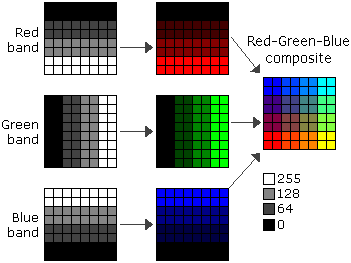
\includegraphics[width=0.5\linewidth]{obrazky-figures/raster-bands.png}
    \caption{\textbf{Rastrové pásma}. Prevzaté z~\cite{arcgis-desktop}.}
    \label{fig:raster-bands}
\end{figure}

\subsubsection{Rastrové formáty}
Pri analýze a~zobrazovaní rastrových dát je potrebné tieto dáta upraviť do~kompaktnejšej formy. To umožňujú rôzne rastrové formáty, ktoré sa starajú o dve úlohy \--- zbaľovanie dát do~pixelov, následné ukladanie vzťahov medzi týmito pixelmi a~ich umiestňovanie na~zemeguľu. Medzi najznámejšie rastrové formáty mapových dát patrí \emph{GeoTIFF}, \emph{JPEG2000} a~\emph{IMG}~\cite{gis-formats}.

\textbf{GeoTIFF}\footnote{\url{https://trac.osgeo.org/geotiff}} je štandardom pre metadáta, ktorý umožňuje vkladanie informácií o georeferenciách do obrázkového súboru. Tieto informácie obsahujú metadáta ako napr. použitá mapová projekcia, použitý súradnicový systém, dátumy, priestorové rozlíšenie a i.

\textbf{JPEG2000}\footnote{\url{https://jpeg.org/jpeg2000}} je systém obrázkového kódovania, ktorý používa kompresné techniky založené na diskrétnej waveletovej transformácii (DWT). Ponúka rýchlejšiu a~kvalitnejšiu kompresiu oproti klasickej JPEG kompresii. Tento formát je vhodný na spracovanie satelitných obrázkov.

\textbf{IMG} súbory používajú hierarchický formát, ktorý môže ukladať informácie napr. o~súbore, o~pozemných kontrolných bodoch a o~type senzora. Každá vrstva rastrového obrázka je súčasťou súbora formátu IMG, ktorý obsahuje informácie o projekcii, štatistikách, atribútoch a~pod.

\section{Vektorové dáta}
Vektorové dáta na rozdiel od rastrových dát obsahujú základné geometrické útvary. Výhodu oproti rastrovým dátam majú takú, že pri hocijakom priblížení nie je možné vidieť pixely. Je to tým, že vektorové dáta sú zložené z geometrických bodov a čiar, ktoré môžu byť v~prípade potreby prevedené na~obrázok.

Vektorové dáta môžu obsahovať viac informácií ako rastrové dáta. Zatiaľ čo rastrové dáta mohli obsahovať iba atribúty o farbe, nepriehľadnosti alebo výške, vektorové dáta môžu obsahovať informácie o tvare. Tvary vektorových dát obsahujú informácie o~vlastnostiach alebo atribútoch, ako napr. počet ľudí, ktorí žijú v danej oblasti, názov mesta reprezentovaného polygónom a pod.

\subsubsection{Vektorové formáty}
Medzi najznámejšie vektorové formáty dát patrí formát \emph{shapefile} vytvorený spoločnosťou ESRI. Tento formát sa ukladá do zariadenia ako skupina aspoň troch súborov, ktoré síce majú rovnaký názov, ale majú rôznu príponu:
\begin{itemize}
    \item hlavný súbor \texttt{*.shp} \--- obsahuje popis geometrie každého záznamu
    \item indexový súbor \texttt{*.shx} \--- prepája prvok v hlavnom súbore so záznamom v atribútovej tabuľke
    \item databázový súbor \texttt{*.dbf} \--- databázový súbor, obsahuje dáta atribútov pre každý záznam
\end{itemize}

Okrem hore zmienených súboroch môže mať \emph{shapefile} aj iné súbory, ktoré obsahujú ďalšie informácie o dátach:
\begin{itemize}
    \item projekčný súbor \texttt{*.prj} \--- ukladá informácie o súradnicovom systéme
    \item priestorové indexy \texttt{*.gix}, \texttt{*.sbn}, \texttt{*.sbx} \--- umožňujú rýchlejšie vyhľadávanie prvkov
    \item atribútové indexy \texttt{*.atx} \--- urýchľujú vyhľadávanie v atribútovej tabuľke
    \item metadátový súbor \texttt{*.shp.xml} \--- metadáta o zvolenom prvku
    \item kódovací súbor \texttt{*.cpg} \--- súbor pre správnu identifikáciu znakov
\end{itemize}

Existuje veľa iných vektorových formátov dát, ktoré sa používajú v~GIS\footnote{Geografický informačný systém} ako napr.~\emph{KML}, \emph{KMZ}, \emph{GPX}, \emph{OSM XML}, \emph{PBF} a~\emph{GeoJSON}~\cite{gis-formats}.

\textbf{KML} (Keyhole Markup Language) je dátový formát vyvinutý pre aplikáciu Google Earth. Okrem ukladania informácií o geometrii obsahuje možnosti konfigurácie pre Google Earth mapy.

\textbf{KMZ} (Keyhole Markup Zipped) je dátový formát, ktorý sa takisto používa v aplikáciách Google. Tento formát je rozšírením KML formátu, pretože obsahuje okrem textového popisu aj obrázky tvoriace 3D vizualizácie prvku.

\textbf{GPX} (GPS Exchange Format) je formát údajov GPS pre ukladanie bodov, trás a ich atribútov. Ukladá informácie pomocou textu, podobne ako súbory typu KML.

\textbf{OSM XML} (OpenStreetMap XML) je dátový formát založený na jazyku XML\footnote{eXtensible Markup Language}. Súbory tohto formátu sú zbierkou vektorových funkcií získaných od~open-source komunity.

\textbf{PBF} (Protocolbuffer Binary Format) je efektívnejší formát OSM XML formátu. Jedná sa o~binárny dátový formát, pretože veľkosť súboru vo~formáte PBF je mnohonásobne menšia ako veľkosť súboru vo~formáte OSM XML.

\textbf{GeoJSON} je formát založený na formáte JSON\footnote{Javascript Object Notation}. Tento formát je navrhnutý pre reprezentáciu jednoduchých priestorových geografických dát a ich atribútov. Pomocou tohto formátu je možné reprezentovať nasledujúce geometrické typy: \emph{Point}, \emph{LineString}, \emph{Polygon}, \emph{MultiPoint}, \emph{MultiLineString} a \emph{MultiPolygon}~\cite{rfc7946}. Vo výpise~\ref{lst:geojson} je možné vidieť, ako je reprezentovaný bod (Point) vo formáte GeoJSON.

\lstset{
    caption={\texttt{FeatureCollection} obsahuje vo vlastnosti \texttt{features} objekt typu \texttt{Feature}, ktorý v \texttt{properties} obsahuje informácie viazané na objekt \texttt{geometry}.},
    label={lst:geojson},
    basicstyle=\ttfamily\footnotesize\bfseries,
    xleftmargin=.2\textwidth, xrightmargin=.2\textwidth
}   
\begin{lstlisting}
{
  "type": "FeatureCollection",
  "features": [
    {
      "type": "Feature",
      "properties": {
        "kraj": "Moravsko-sliezsky",
      },
      "geometry": {
        "type": "Point",
        "coordinates": [
          17.60100156068802,
          49.196293610455584
        ]
      }
    }
  ]
}
\end{lstlisting}


\section{Geografické súradnice}
Najbežnejším spôsobom ako je možné ukladať miesta na Zemi je pomocou geografických súradníc. Geografické súradnice súhrnne označujú zemepisnú šírku a zemepisnú dĺžku. Ide o~dve uhlové súradnice, ktoré sú vztiahnuté k Zemi alebo k~jej náhradnému telesu, pomocou ktorých možno určiť ľubovoľnú polohu tohto bodu na Zemi~\cite{pyramida1987}. Môžu byť reprezentované v~šesťdesiatkovej sústave ako napr.~$31$\textdegree\, $42$\textquotesingle, ale nový štandard umožňuje reprezentovať tieto čísla ako reálne čísla t.j.~$31,7$.

\textbf{Zemepisná šírka} je uhol medzi zvislicou miesta na zemský povrch a rovinou rovníka. Vyjadruje sa na mapách rovnobežkami. Je to hodnota v intervale $\langle-180$; $180\rangle$.

\textbf{Zemepisná dĺžka} je uhol medzi rovinou základného poludníka a rovinou poludníka daného bodu. Vyjadruje sa na mapách poludníkmi. Je to hodnota v intervale $\langle-90$; $90\rangle$.


\section{Geografický objekt}
Väčšinu geografických dát je možné reprezentovať tromi typmi geografických objektov: body, čiary a~polygóny~\cite{geographicobjects}. Na~obrázku~\ref{fig:geo-objects} je vidieť popis geometrických objektov a~ako je možné ich využiť.

\begin{figure}[ht]
    \centering
    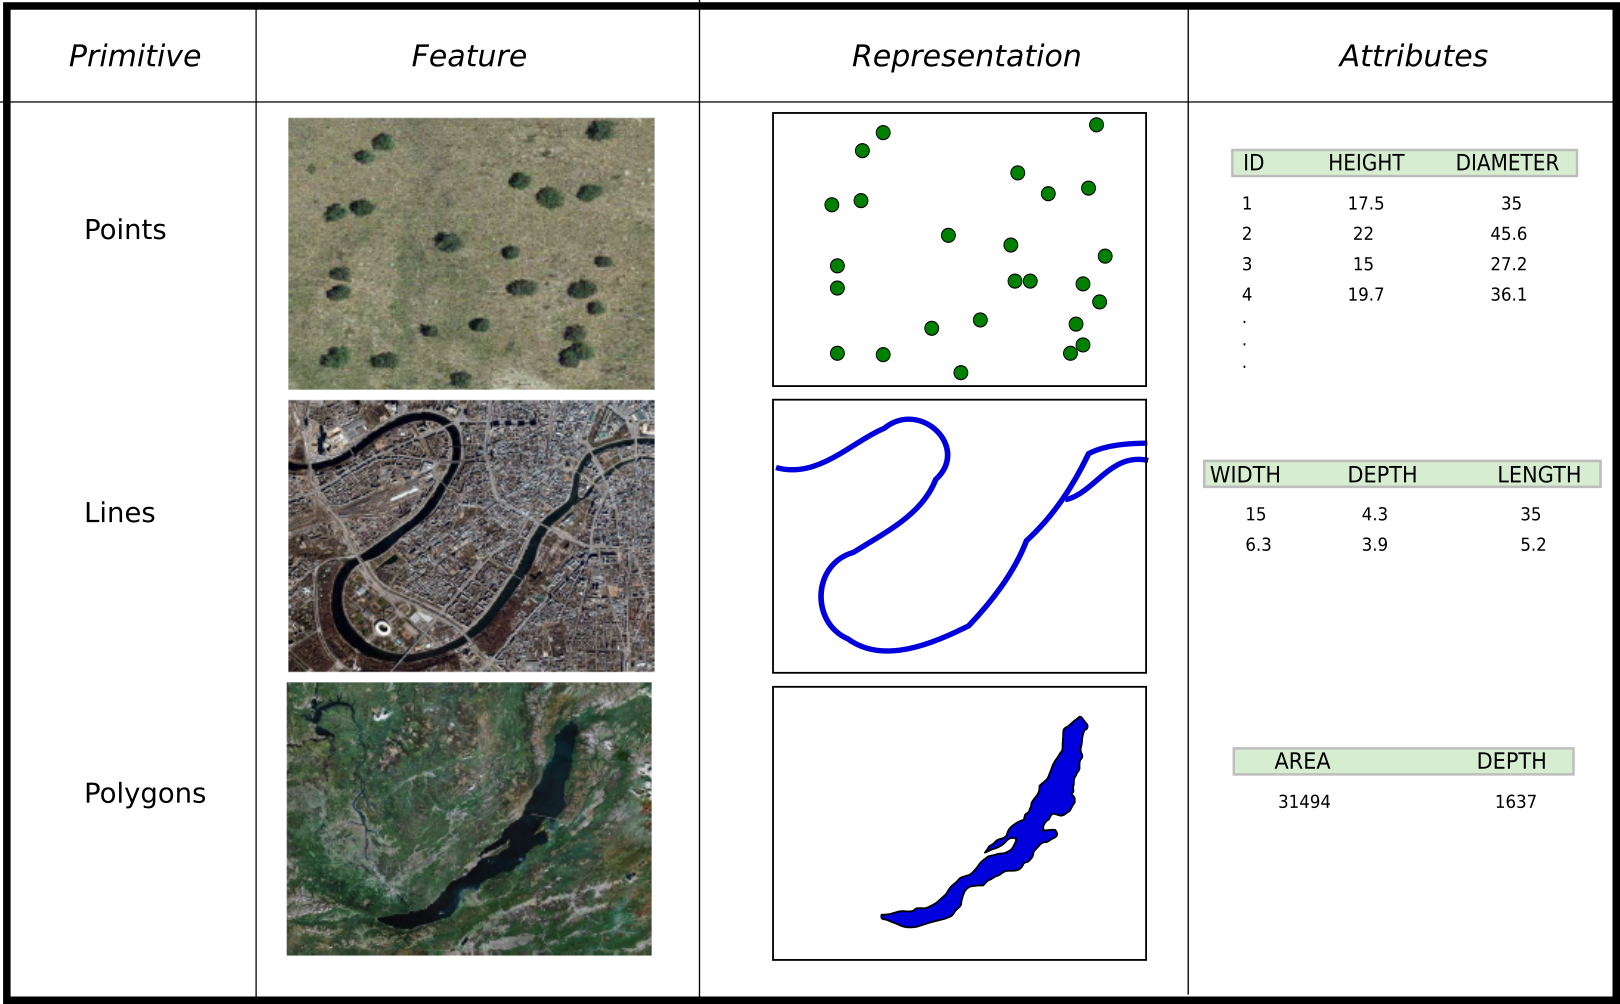
\includegraphics[width=0.8\linewidth]{obrazky-figures/geo-objects.png}
    \caption{Geografické objekty, ich reprezentácia, príklady a možné atribúty. Prevzaté z~\cite{introductiontogis}.}
    \label{fig:geo-objects}
\end{figure}

\textbf{Bod} (point) reprezentuje jednotlivý pár súradníc X, Y. Body sú bežne používané na~vizualizáciu udalostí a~javov, ktoré môžu byť identifikované špeciálnymi polohami na~mape (napr. supermarket, kostol).

\textbf{Čiara} (line) reprezentuje množinu usporiadaných bodov \--- uzlov, ktoré sú pospájané do~čiary. Tieto geometrické útvary majú jednoznačne zadefinovaný začiatočný a~koncový bod (napr. cesta, rieka).

\textbf{Polygón} (polygon) reprezentuje množinu usporiadaných bodov \--- uzlov, ktoré sú navzájom pospájané líniami do uzatvorenej plochy. Majú regionálny alebo zónový rozsah ohraničený súborom mapovateľných hraníc (napr. regióny).\\

Použitím bodov, čiar a polygónov môže byť geografický priestor modelovaný priradením hodnôt k týmto objektom. Každá časť mapy môže obsahovať viacero objektov. Napríklad pri vytváraní mapovej vrstvy s krajinami sveta by bolo potrebné, aby pre krajinu USA bolo vytvorených viacero polygónov (kontinentálna časť USA, Aljaška, Havajské ostrovy,~a~pod.). Všetky tieto polygóny vytvárajú jeden prvok, pretože sú súčasťou jednej krajiny a budú zdielať rovnaké priradené hodnoty~\cite{introductiontogis}.

Pri reprezentovaní špecifického prvku alebo javu na~mape nie je vždy jednoznačné, ktorý typ geografického objektu by sa mal použiť. Rovnaký geografický jav môže reprezentovať rôzne typy geografických objektov pri rôznych úrovniach priblíženia. Napríklad mesto môže byť reprezentované ako bod na~mape, ale takisto môže byť reprezentované polygónom~\cite{geographicobjects}.



\chapter{Zdroje mapových dát}
\label{chap:source-map-data}
Mapové dáta sa dajú získať z viacerých zdrojov. Každý takýto zdroj má svoje výhody aj nevýhody. Táto kapitola oboznámi čitateľa z akých zdrojov je možné získať mapové dáta, aké sú možné výhody a aké sú nevýhody daného zdroja, ale aj aké formáty súborov mapových dát tieto zdroje ponúkajú. 


\section{GIS}
Geografický informačný systém (GIS) je informačný systém, ktorý sa využíva na získavanie, analyzovanie, vizualizáciu a manažment dát s~priestorovým alebo mapovým vyjadrením. GIS spracováva geografické údaje v~digitálnej podobe. Časť takýchto údajov vzniká napr. pomocou satelitných údajov, meraním pomocou polohového systému GPS alebo inými meracími prístrojmi. Údaje v~papierovej podobe je nutné digitalizovať. Súčasťou GIS je hardvér (počítače, servery, zariadenia na zber dát,...), softvér (špecializované programy pre prácu s~priestorovými dátami), dáta (priestorové údaje) a~používatelia (spracovatelia dát, administrátori GIS a~prijímatelia priestorových informácií)~\cite{introductiontogis}. Používatelia systému môžu využívať rôzne metódy spracovania geografických údajov, ktoré umožňujú údaje prehľadávať, triediť, reklasifikovať, transformovať a~modelovať~\cite{hofierka2003gis}.

Geografické dáta v GIS môžu byť organizované dvomi základnými modelmi \--- vektorovým a rastrovým modelom~\cite{holman2014priestorovedata}.

\subsection*{Vektorový model}
Vektorový model je nazývaný podľa spôsobu vyjadrenia jeho jednotlivých častí \--- úseky kriviek s definovanou veľkosťou a smerom \--- \emph{vektorom}. Vektorový model GIS pracuje s~tromi variantami geografických objektov \--- bod, čiara a polygón.

Existujú rôzne modely dát pomocou ktorých je možné reprezentovať geografické objekty s~využitím vektorovej grafiky:
\begin{itemize}
    \item \textbf{Špagetový model} \--- vychádza z postupov využívaných pri digitalizácií máp. Každý objekt na mape je reprezentovaný jedným záznamom a je uložený ako reťazec X, Y súradníc. Z tohto modelu nie je možné získať žiadne informácie o vzťahoch medzi jednotlivými subjektami aj keď sa jedná o priestorové dáta.
    \item \textbf{Topologický model} \--- každá línia tohto modelu začína a končí v~uzle. Všetky informácie tohto modelu sú ukladané do tzv. \emph{topologických tabuliek} \--- tabuľka spojov, súradníc a polygónov. Model vďaka tomu uchováva priestorové vzťahy medzi objektami.
    \item \textbf{Hierarchický model} \--- ukladá zvlášť informáciu o bodoch, líniách a plochách v~hierarchickej štruktúre pre jednoduchšie vyhľadávanie v dátach. V modeli sú takisto zahrnuté aj odkazy medzi jednotlivými druhmi objektov a obsahuje topologickú informáciu. Tento model je pre manipuláciu a vyhľadávanie v dátach najvhodnejší.
\end{itemize}

\subsection*{Rastrový model}
Rastrová reprezentácia mapových dát sa na rozdiel od vektorovej zameriava na zemský povrch. Používa sa skôr na javy ako je napr. úhrn zrážok či nadmorská výška.

Základným princípom tohto formátu je pokrytie zemského povrchu pravidelnou alebo nepravidelnou sieťou, pričom jednotka tejto siete je \emph{bunka} (pixel, cell). Nepravidelná sieť má výhodu oproti nepravidelnej siete takú, že pomocou nepravidelnej siete je možné jednoduchšie reprezentovať rôzne prechody z roviny na terénnu hranu. Na druhú stranu použitie nepravidelnej siete je výpočtovo a aj algoritmicky náročnejšie. Keďže v tomto modeli neexistujú objekty známe z vektorového modelu GIS, bunky definujú vlastnú hodnotu sledovaného javu v konkrétnej časti priestoru. Hodnota v jednej bunke odpovedá bodu, rada spojených buniek s rovnakou hodnotou odpovedá línii a skupina navzájom susediacich buniek odpovedá ploche.

\begin{figure}[ht]
    \centering
    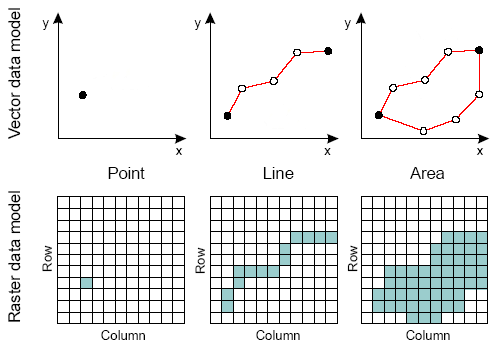
\includegraphics[width=0.5\linewidth]{obrazky-figures/vector-and-raster-data.png}
    \caption{\textbf{Vektorový a rastrový dátový model}. Prevzaté z~\cite{jukil2017mapdata}.}
    \label{fig:vectorandraster}
\end{figure}

\subsection*{ArcGIS}
V súčasnosti existujú rôznorodé softvéry pre GIS. Medzi najznámejšie patrí ArcGIS od~spoločnosti ESRI, ktorý slúži na mapovanie a priestorovú analýzu navrhnutý tak, aby podporoval poslanie a obchodné ciele organizácií. Tento systém poskytuje tri úrovne licencií. Typ zvolenej licencie rozhoduje o tom, ako sú uložené dáta a ako je možné ich editovať. 

Medzi najznámejšie aplikácie systému ArcGIS patrí ArcMap (použiteľná na priestorové analýzy, editáciu dát a tvorbu kartografických výstupov), ArcCatalog (pomáha organizovať a spravovať všetky dáta), ArcGIS Explorer (voľne dostupný prehliadač priestorových dát), ArcGIS for~Server (serverové riešenie pre GIS, umožňuje jednoduchú konfiguráciu webových aplikácií a poskytuje kompletné vývojárske prostredie pre \emph{.NET} a \emph{Java}).

\subsection*{ArcČR 500}
ArcČR 500~\cite{arcgis} je digitálna vektorová geografická databáza Českej republiky, spracovaná na úrovni podrobnosti 1 : \numprint{500000}. Obsahom databázy sú prehľadné geografické informácie o~ČR. Zdrojom dát pre geografické dáta ArcČR 500 v 3.3 je databáza Data200, čo je národná vektorová geografická databáza Zeměměřického úřadu (ZÚ) odpovedajúca presnosťou a~stupňom generalizácie 1 : \numprint{200000}. Vstupné dáta z Data200 majú deklarovanú absolútnu presnosť do 100 m. Absolútna polohová odchýlka ArcČR 500 v 3.3 je odhadovaná do 200~m.

Dáta sú uchovávané iba v GIS formátoch firmy ESRI a to vo formáte súborovej databázy. ArcČR 500 je zložená z dvoch geodatabází \--- geografické prvky a administratívne členenie.\\

\textbf{Geografické prvky} ArcČR 500 boli odvodené zo 17-tich vrstiev databázy Data200. Vrstvy súborovej databázy \texttt{ArcCR500\_v33.gdb} ako aj ich popis a typ prvkov je možné vidieť v tabuľke~\ref{tab:arccr500}.

\begin{table}[H]
\caption{Súborová databáza ArcCR500\_v33.gdb. Prevzaté z~\cite{arcgis}.}
\label{tab:arccr500}
\centering
\begin{tabular}{|l|p{0.5\linewidth}|l|}
    \hline
    \textbf{vrstva}        & \textbf{popis}                                 & \textbf{typ prvku} \\ \hline
    Letiste                & Letisko                                        & bod                \\
    SidlaBody              & Sídla nad 500 obyvateľov                       & bod                \\
    VyskoveKoty            & Výškové kóty (vrcholy kopcov)                  & bod                \\
    ZeleznicniStanice      & Železničná stanica                             & bod                \\
    Hranice                & Štátna, krajská a okresná hranica              & línia              \\
    Silnice                & Cesta                                          & línia              \\
    VodniToky              & Vodné toky                                     & línia              \\
    Vrstevnice             & Vrstevnice po 25 m                             & línia              \\
    Zeleznice              & Železnice                                      & línia              \\
    BazinyARaseliniste     & Močiar a rašelinisko väčšie ako 30 ha          & polygón            \\
    Lesy                   & Lesné plochy väčšie ako 30 ha                  & polygón            \\
    SidlaPlochy            & Sídla nad \numprint{5000} obyvateľov           & polygón            \\
    VodniPlochy            & Vodné plochy väčšie ako 15 ha                  & polygón            \\
    ChranenaUzemi          & Národné parky a chránené krajinné oblasti      & polygón            \\
    KladyZakladnichMap     & Klady základných máp ČR                        & polygón            \\
    KladyTopografickychMap & Klady vojenských topografických máp            & polygón            \\
    SouradnicovaSitJTSK    & Súradnicová sieť systému JTSK v intervale 1~km & línia              \\
    ZemepisnaSitETRS89     & Zemepisná sieť v systéme ETR89                 & línia              \\
    ZemepisnaSitWGS84      & Zemepisná sieť v systéme WGS84                 & línia              \\
    DigitalniModelReliefu  & Raster digitálneho modelu reliéfu              & raster             \\
    StinovanyRelief        & Raster tieňovaného modelu reliéfu              & raster             \\ \hline
\end{tabular}
\end{table}

Každá vrstva tejto databázy môže nadobúdať rôzne hodnoty atribútov, ktoré sú pre danú vrstvu zadefinované. V tejto práci sú uvedené pre ilustráciu iba vrstvy Letisko (tabuľka~\ref{tab:letisko}) a Hranica (tabuľka~\ref{tab:hranica}). V tabuľke \ref{tab:letisko} je možné vidieť, že atribút \texttt{TYP} môže nadobúdať tri hodnoty \--- t.j.~letisko je buď civilné alebo vojenské, alebo civilné a vojenské. Táto vrstva je zobrazená na mape ako bod. Na druhú stranu vrstva \emph{Hranica}, ktorá sa zobrazuje na mape ako línia, nemá takú variabilitu atribútov ako vrstva \emph{Letisko}. V tabuľke~\ref{tab:hranica} je možné vidieť, že daná vrstva má iba jeden zadefinovaný atribút, ktorý ale môže nadobúdať 3 hodnoty \--- t.j. hranica môže byť štátna, krajská alebo okresná.

\begin{table}[H]
\caption{Vrstva Letisko (Letiste). Prevzaté z~\cite{arcgis}.}
\label{tab:letisko}
\centering
\begin{tabular}{|l|l|l|}
    \hline
    \textbf{meno atribútu}         & \textbf{popis}      & \textbf{nadobúdané hodnoty}   \\ \hline
    \textbf{TYP}          & Typ letiska         & \begin{tabular}[c]{@{}l@{}}1 - civilné\\ 2 - vojenské\\ 3 - civilné a vojenské\end{tabular} \\
    \textbf{NAZEV}        & Meno                & \textit{konkrétne meno}       \\
    \textbf{NAZEV\_ASCII} & Meno (ASCII formát) & \textit{konkrétne meno}       \\
    \textbf{ICAO}         & Kód ICAO            & \textit{konkrétny kód}        \\
    \textbf{STATUT}       & Statut letiska      & \begin{tabular}[c]{@{}l@{}}1 - medzinárodné\\ 2 - vnútroštátne\end{tabular}                 \\ \hline
    \end{tabular}
\end{table}

\begin{table}[H]
\caption{Vrstva Hranica (Hranice). Prevzaté z~\cite{arcgis}.}
\label{tab:hranica}
\centering
\begin{tabular}{|l|l|l|}
    \hline
    \textbf{meno atribútu} & \textbf{popis} & \textbf{nadobúdané hodnoty}  \\ \hline
    \textbf{TYP}  & Typ hranice    & \begin{tabular}[c]{@{}l@{}}1 - štátna\\ 2 - krajská\\ 3 - okresná\end{tabular} \\ \hline
\end{tabular}
\end{table}

Dáta z Českého statistického úřadu (ČSÚ) boli použité pre tvorbu dát \textbf{administratívneho členenia}. Vrstvy súborovej geodatabázy \texttt{AdministrativniCleneni\_v13.gdb} ako aj ich popis sa nachádza v tabuľke~\ref{tab:administrativne-clenenie}.
\begin{table}[H]
\caption{Súborová databáza AdministrativniCleneni\_v13.gdb. Prevzaté z~\cite{arcgis}.}
\label{tab:administrativne-clenenie}
\centering
\begin{tabular}{|lll|}
    \hline
    \textbf{názov}  & \textbf{popis}                 & \textbf{typ prvku} \\ \hline
    \textbf{ZSJ}    & Základné sídelné jednotky      & bod/polygón        \\
    \textbf{UTJ}    & Územné technické jednotky      & bod/polygón        \\
    \textbf{KU}     & Katastrálne územie             & bod/polygón        \\
    \textbf{MOaMC}  & Mestské obvody a mestské časti & bod/polygón        \\
    \textbf{COB}    & Časti obce                     & bod/polygón        \\
    \textbf{OBCE}   & Obce a vojenské újazdy         & bod/polygón        \\
    \textbf{POU}    & Obce s povereným úradom        & bod/polygón        \\
    \textbf{ORP}    & Obce s rozšírenou pôsobnosťou  & bod/polygón        \\
    \textbf{OKRESY} & Okresy                         & bod/polygón        \\
    \textbf{KRAJE}  & Kraje                          & bod/polygón        \\
    \textbf{STAT}   & Štát                           & bod/polygón        \\ \hline
\end{tabular}
\end{table}


\section{OpenStreetMap}
OpenStreetMap~\cite{openstreet} je projekt, ktorý vznikol za účelom vytvárania geografickej databázy celého sveta. Cieľom tohto projektu je mať časom záznam o každom geografickom prvku na~planéte. Zatiaľ čo to začalo mapovaním ulíc, postupom času tento projekt zahŕňa chodníky, budovy, vodné cesty, potrubia, lesy, pláže, poštové schránky a dokonca aj jednotlivé stromy.

\begin{figure}[ht]
    \centering
    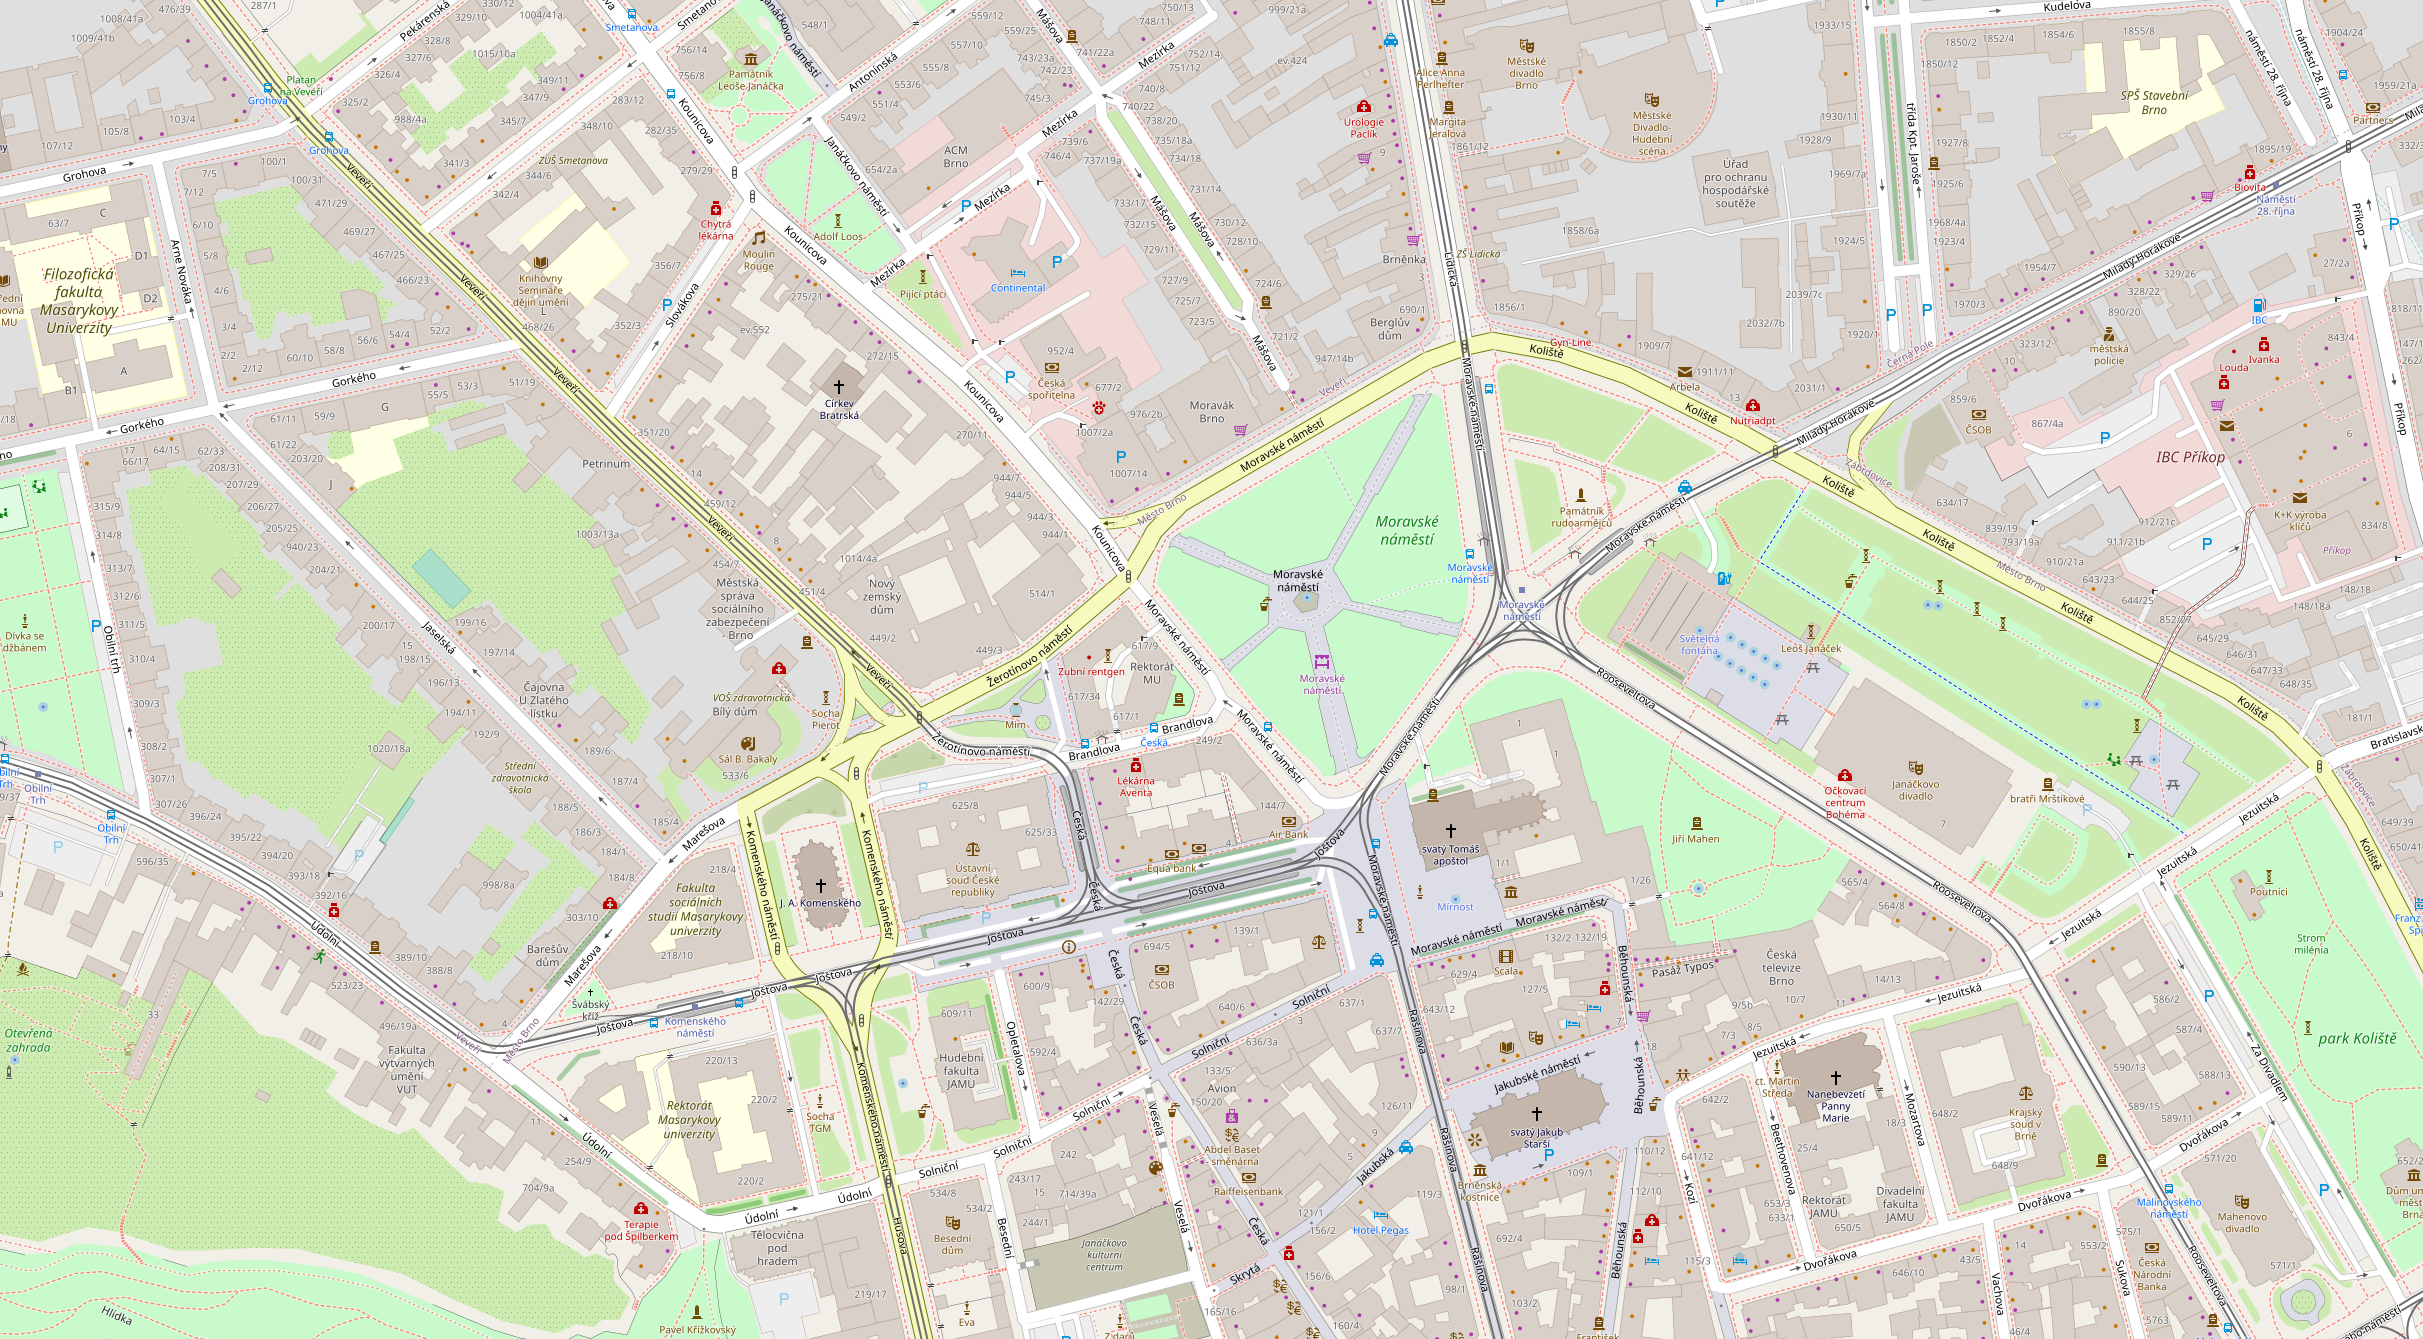
\includegraphics[width=\linewidth]{obrazky-figures/openstreetmap.png}
    \caption{\textbf{OpenStreetMap}. Výsek z mapy časti Brna.}
    \label{fig:openstreetmap}
\end{figure}

\subsection*{História projektu}
Projekt OpenStreetMap má svoj začiatok v auguste v roku 2004, kedy britský programátor Steve Coast experimentoval s USB GPS prijímačom. Použil softvér nazývaný GPSDrive, ktorý bral mapy z Microsoft MapPoint, ale porušoval licenčné podmienky. Coast vedome nechcel porušovať autorské práva týchto máp, preto hľadal alternatívu, ktorá by neporušovala licenčné podmienky, tú ale nenašiel. Zistil, že neexistujú zdroje mapových dát, ktoré by mohol používať v otvorenom softvére bez toho, aby porušoval licenčné podmienky alebo platil obrovské sumy peňazí. Po odprezentovaní jeho nápadu o vytvorení vlastnej mapy na konferencii otvorených softvérov v Londýne zistil, že viacerí ľudia mali podobný nápad alebo ich Coastov nápad zaujal, a tak vznikla skupina OpenStreetMap.

V začiatkoch bol dátový model príliš simplistický, pretože obsahoval iba jednoduché čiary nakreslené cez informácie Landsat od NASA. V marci v roku 2006 bola vytvorená prvá editovacia aplikácia pre OpenStreetMap \--- JOSM\footnote{\url{https://josm.openstreetmap.de}}. Po chvíli bola v tomto roku vytvorená prvá plnofarebná mapa mesta Weybridge. V máji toho roku sa usporiadala prvá spoločná akcia, na ktorej bolo úlohou zmapovať ostrov Wight. Bolo to prvýkrát, kedy sa stretlo viacero mapovačov a znamenalo to pre nich prelomový bod projektu, pretože bola vytvorená detailná mapa. Takéto akcie OpenStreetMap komunity sa začali konať častejšie a boli usporadúvané po celom svete.

V auguste v roku 2006 bola vytvorená nadácia \emph{OpenStreetMap Foundation}, ktorou úlohu je podporovať, ale nie kontrolovať OpenStreetMap projekt. Venuje sa podpore rastu, rozvoja a distribúcii voľne dostupných geografických dát a poskytovaniu geografických údajov komukoľvek na používanie a zdieľanie.

Serverový softvér bol pôvodne napísaný v programovacom jazyku Java, ale v~máji v~roku 2007 bola implementácia softvéru prepísaná do platformy Ruby on Rails\footnote{\url{https://rubyonrails.org}}. Časom ako začal projekt postupne narastať, začali svojimi dátami prispievať súkromné spoločnosti, mestá, ale aj štáty~\cite{bennett2010openstreetmap}. Vo februári v roku 2008 bolo zaregistrovaných \numprint{25000} užívateľov na~stránke OpenStreetMap, v marci v roku 2009 to už bolo \numprint{100000} užívateľov. Počet užívateľov stále rastie, v čase písanie tohto textu je to už viac ako 8,3 milióna zaregistrovaných užívateľov.

\subsection*{Dátový model OpenStreetMap}
Prvky (anglicky elements) sú základnou stavebnou súčasťou dátového modelu OpenStreetMap slúžiace k popisu reálneho sveta. Medzi základné prvky OpenStreetMap projektu patria uzol, cesta a relácia. Tieto prvky je možné popísať značkami.

\textbf{Uzol\footnote{\url{https://wiki.openstreetmap.org/wiki/Node}}} (anglicky node) označuje konkrétny bod na povrchu Zeme, je určený svojou zemepisnou šírkou a dĺžkou. Skladá sa minimálne z dvojice súradníc a svojho jednoznačného identifikačného čísla (id).

\textbf{Cesta\footnote{\url{https://wiki.openstreetmap.org/wiki/Way}}} (anglicky way) je usporiadaný zoznam 2 až \numprint{2000} uzlov, ktoré definujú lomenú čiaru. Cesta má aspoň jednu značku alebo je vložená do relácie.

\textbf{Relácia\footnote{\url{https://wiki.openstreetmap.org/wiki/Relation}}} (anglicky relation) sa skladá z jednej alebo viacerých značiek a usporiadaného zoznamu jedného alebo viacerých uzlov alebo ciest. Každý prvok relácie je tzv. člen (anglicky member). Používa sa k popisu závislosti medzi rôznymi prvkami. Každý člen relácie môže voliteľne mať nejakú rolu, ktorá popisuje jeho význam v rámci relácie.

\textbf{Značka\footnote{\url{https://wiki.openstreetmap.org/wiki/Tags}}} (anglicky tag) sa skladá z kľúča a hodnoty. Každá značka popisuje určitú vlastnosť dátových prvkov (uzlov, ciest a relácií) alebo sadu zmien. Kľúč popisuje tému, kategóriu alebo typ mapového prvku (napr. cesta \--- \emph{highway} alebo názvy \--- \emph{name}). Hodnota konkretizuje vlastnosť, ktorú všeobecne popisuje kľúč. Napríklad značka \texttt{highway=residential} predstavuje cestu, ktorá vedie obytnou oblasťou.

\begin{figure}[ht]
    \centering
    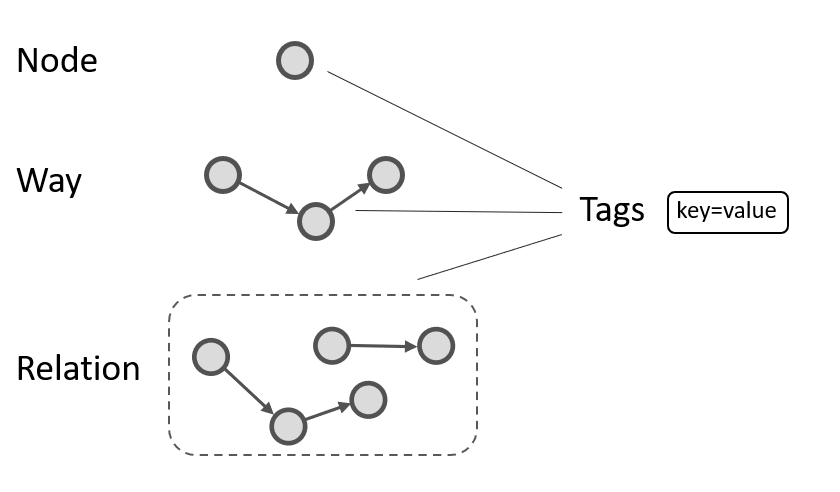
\includegraphics[width=0.7\linewidth]{obrazky-figures/openstreetmap-datamodel.png}
    \caption{\textbf{Dátový model OpenStreetMap}. Prevzaté z~\cite{jafari2022building}.}
    \label{fig:osmdatamodel}
\end{figure}

\subsection*{Sťahovanie dát}
Sťahovať mapové dáta z~databázy OpenStreetMap je možné viacerými spôsobmi. Vhodná voľba sťahovania dát závisí od toho, aké veľké množstvo dát sa rozhodneme sťahovať.

Pre veľké oblasti je vhodnou voľbou si stiahnuť dáta lokálne. Stiahnuť databázu celého sveta je možné na stránke Planet.osm\footnote{\url{https://planet.openstreetmap.org}}. Z tejto stránky je možné stiahnuť databázu celého sveta vo formáte OSM XML alebo PBF. Táto databáza je aktualizovaná každý týždeň a~aktuálne (1. 5. 2022) veľkosť súboru vo~formáte OSM XML má $115$~GB a vo~formáte PBF má veľkosť $63$~GB.

Pre menšie oblasti je tiež možné použiť hore zmienené nástroje, avšak okrem toho je možné vybrať oblasť pomocou ohraničeného boxu, ktorý je zložený z~minimálnej a~maximálnej zemepisnej dĺžky a~zemepisnej šírky. Pomocou týchto hodnôt je možné vytvoriť URL s~HTTP API požiadavkou. Ohraničený box v~URL je vyjadrený ako štyri hodnoty za sebou, oddelené čiarkami. Vo~výpise~\ref{lst:osm-api} je možné vidieť príklad URL s~HTTP API požiadavkou. Hodnoty v~parametri \texttt{bbox} sú zoradené v~poradí: minimálna zemepisná šírka, minimálna zemepisná dĺžka, maximálna zemepisná šírka, maximálna zemepisná dĺžka.

\lstset{
    caption={Príklad HTTP API požiadavku.},
    label={lst:osm-api},
    basicstyle=\ttfamily\normalsize\bfseries,
    xleftmargin=.04\textwidth, xrightmargin=.4\textwidth
}
\begin{lstlisting}
https://api.openstreetmap.org/api/0.6/map?bbox=16.61,49.22,16.63,49.23
\end{lstlisting}

Ďalšou možnosťou je použiť stránku Geofabrik\footnote{\url{https://download.geofabrik.de}}, ktorá umožňuje sťahovať väčšie aj~menšie oblasti podľa kontinentov, štátov, provincií alebo miest. Stiahnuté súbory z~tejto stránky môžu byť vo~formáte \texttt{osm.pbf}, \texttt{shp.zip} alebo \texttt{osm.bz2}.

\section{Kataster}
Kataster predstavuje register resp. zoznam a používa sa vo viacerých významoch:
\begin{itemize}
    \item súpis nehnuteľného majetku, ktorý bol vytvorený pre daňové a úradné účely
    \item kataster nehnuteľností, katastrálna kniha
    \item katastrálne územie
\end{itemize}

\subsection*{Kataster nehnuteľností}
Súčasný kataster nehnuteľností~\cite{baudys-katastranemovitosti} na území Českej republiky mal ekvivalent medzi svojimi právnymi predchodcami \--- tzv.~pozemkovú knihu, ktorá slúžila na majetkoprávne účely. Okrem pozemkovej knihy sa používal aj pozemkový kataster, ktorý slúžil na~daňové účely. Pozemkový kataster sa používal približne do roku 1957 a zapisovanie do~pozemkovej knihy bol ukončený v~roku 1964, pretože nevypovedala o~skutočných a~aktuálnych právnych vzťahoch k~nehnuteľnostiam. Preto bola vytvorená nová pozemková evidencia nehnuteľností, ktorej hlavným účelom bolo zaistiť podklady pre plánovanie národného hospodárstva. Táto evidencia bola vedená až do roku 1992, kedy si spoločenské zmeny vyžiadali založenie dnešného katastru nehnuteľností.

Dnešný kataster nehnuteľností plní úlohu pozemkovej knihy aj pozemkového katastru a slúži aj ako podklad pre geografické informačné systémy. Kataster nehnuteľností je definovaný ako súbor údajov o nehnuteľností v Českej republike. Okrem súpisu a popisu nehnuteľností zahŕňa ich geometrické a polohové určenie pre jednu katastrálnu obec alebo katastrálne územie. Aj keď v českom katastri sú zapísané všetky pozemky, zo stavieb sú zapísané v katastri len tie budovy, ktoré stanovuje katastrálny zákon. Ide o budovy s popisným či evidenčným číslom alebo hlavnú budovu v rámci areálu nehnuteľností. Na obrázku~\ref{fig:katastrmapa} je možné vidieť ako vyzerá katastrálna mapa mestskej časti Brno-Královo Pole. Obrázok je exportovaný zo stránky Českého katastru nemovitostí\footnote{\url{https://nahlizenidokn.cuzk.cz/VyberKatastrMapa.aspx}}, ktorý okrem faktických a právnych informácií o nehnuteľnostiach obsahuje katastrálne mapy a informácie o vlastníkoch nehnuteľností.

\begin{figure}[ht]
    \centering
    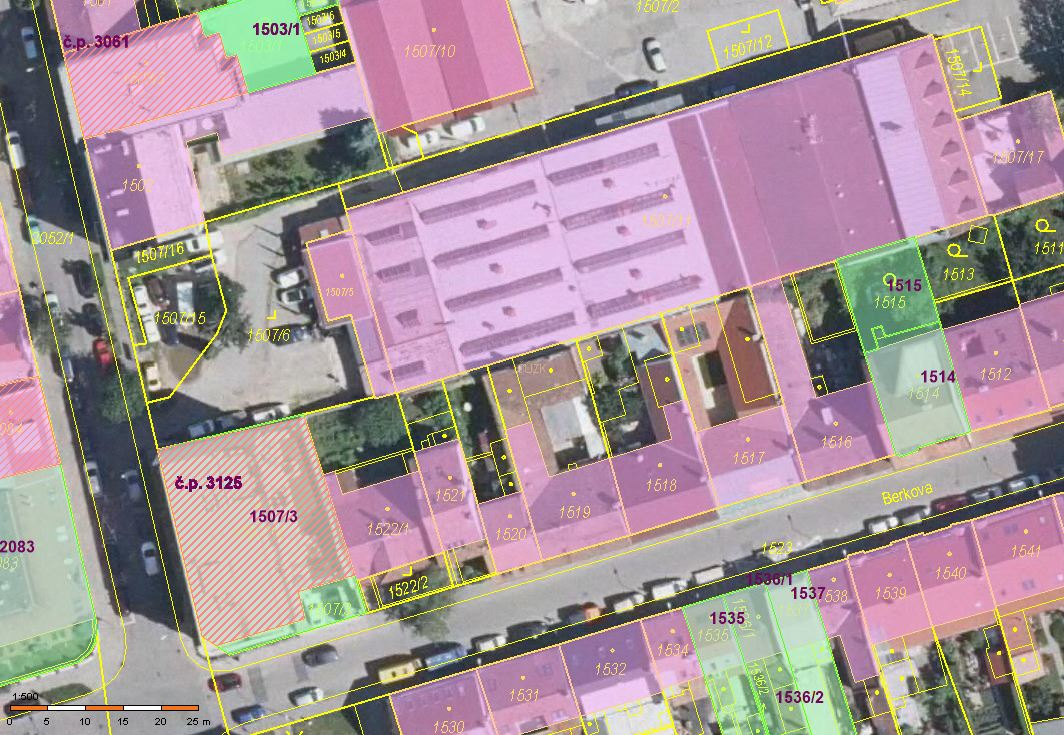
\includegraphics[width=0.8\textwidth]{obrazky-figures/katastr-ortofo-kralovopole.jpg}
    \caption{\textbf{Katastrálna mapa s ortofotomapou mestskej časti Brno-Královo Pole}. Ružová farba predstavuje budovy, budovy so zelenou farbou sú nehnuteľnosti s~cenovými údajmi k~jednotke (byty alebo nebytové priestory), vyšrafované budovy sú nehnuteľnosti s~cenovými údajmi k~parcele.}
    \label{fig:katastrmapa}
\end{figure}

\subsection*{Územný plán}
Vlastníci katastrov nehnuteľností si musia byť istý, že na danom území existuje poriadok, ktorý by mal zaručovať, že ich práva nebudú ohrozované náhodnými a~meniacimi sa rozhodnutiami. Územným plánovaním sa predchádza nekoncepčnému a zložitému rozvoja obce. Zaoberá sa všetkými aspektmi nášho prostredia. Ide prevažne o~stavbu sídiel, dopravnú a~ technickú infraštruktúru, ale aj o prvky, ktoré vytvárajú prírodné zložky životného prostredia~\cite{uzemnyplan}.



\chapter{Návrh}
\label{chap:navrh}
V tejto kapitole je popísaný návrh systému, na ktorom je založená celá aplikácia. Na začiatku tejto kapitoly sa analyzujú požiadavky na aplikáciu a popisujú kľúčové vlastnosti, ktoré musia byť splnené. Táto kapitola zahŕňa aj bližšie popísanie použitých technológií a~dôvody, prečo boli zvolené dané technológie pri návrhu aplikácie.


\section{Analýza požiadavkov}
\label{sec:analysis}
Požiadavky sú potrebné pri akomkoľvek návrhu aplikácie. S požiadavkami sa treba zamyslieť, ako sa dajú navrhnúť a implementovať. Primárnym cieľom tejto bakalárskej práce je vytvoriť aplikáciu, ktorá na základe získaných dát vytvorí odhady pravdepodobnosti výskytu osôb. Túto aplikáciu je možné vytvoriť tak, aby ju bolo možné v budúcnosti rozšíriť o viaceré funkcionality, ale aj aby bola užívateľsky prívetivá.

Prvou požiadavkou pri vytvorení aplikácie je spracovanie vstupných dát získaných od~užívateľa. Vstupné dáta je možné rozdeliť na dva typy: súradnice a hodnoty pravdepodobností. Druhou požiadavkou je vytváranie a~zobrazovanie heat vrstvy na~mape.

\subsection*{Vstupné súradnice}
Prvým typom vstupných dát sú súradnice, ktoré užívateľ bude môcť zadať rôznymi spôsobmi. Spôsoby získavania vstupných súradníc budú inšpirované získavaním hraničných súradníc na~stránke projektu OpenStreetMap.

Jednou z možností je využitie knižnice \texttt{Leaflet.draw}. Užívateľ v navrhovanej aplikácií by mal byť schopný vykresliť na mapu plochu, z~ktorej by chcel zistiť, aká je pravdepodobnosť výskytu osôb v~danej oblasti. Z~tejto nakreslenej plochy sa dá zistiť, aké sú hranice danej plochy, t.j. aká je minimálna a~maximálna hodnota zemepisnej dĺžky a~aká je minimálna a~maximálna hodnota zemepisnej šírky nakreslenej plochy. Tento spôsob získavania vstupných dát je zobrazený na obrázku~\ref{fig:osm-export}.

Druhá možnosť získavania vstupných súradníc, takisto používaná na stránke projektu OpenStreetMap, by mohla fungovať na základe získavania hraníc mapy, ktorá je na stránke zobrazená. To znamená, že horná a dolná hranica mapy predstavujú zemepisné dĺžky, ľavá a pravá hranica mapy predstavujú zemepisné šírky.

Tretiu možnosť získavania vstupných súradníc je možné použiť v kombinácií s~už zmienenými možnosťami. Užívateľ by mal byť schopný zadať všetky štyri hraničné súradnice manuálne. Pri návrhu takejto možnosti je potrebné myslieť na~to, že súradnica hornej (severnej) hranice musí byť väčšia ako súradnica dolnej (južnej) hranice a súradnica pravej (východnej) hranice musí byť väčšia ako súradnica ľavej (západnej) hranice.

\begin{figure}[ht]
    \centering
    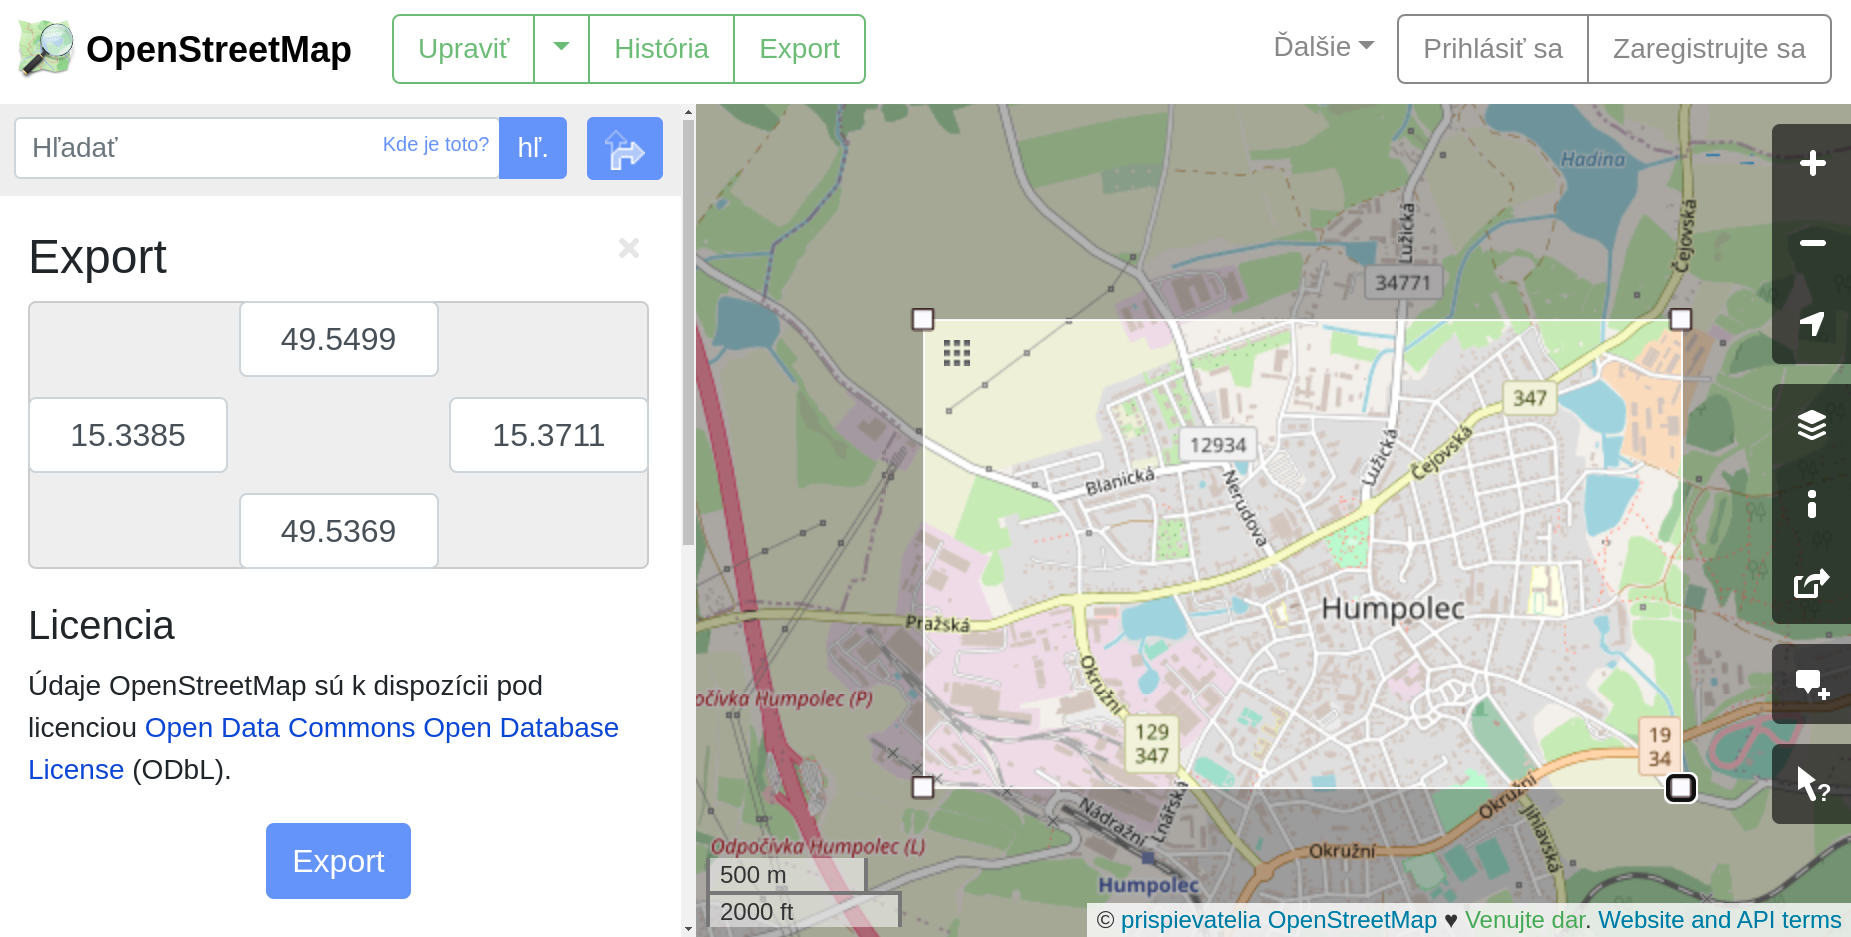
\includegraphics[width=0.8\textwidth]{obrazky-figures/openstreetmap-export.png}
    \caption{Export dát na stránke projektu OpenStreetMap.}
    \label{fig:osm-export}
\end{figure}
    
\subsection*{Hodnoty pravdepodobností}
Druhým typom vstupných dát od užívateľa sú hodnoty pravdepodobností resp.~intenzít pre~značky. Vo~väčšine prípadoch počet týchto vstupných hodnôt pravdepodobností môže byť aj viac ako 100, preto vhodným návrhom pre zadávanie hodnôt je použitie externého súboru. V tomto súbore by mal užívateľ mať možnosť zadefinovať, ktoré značky by sa mali použiť pri vykresľovaní heat vrstvy a aké hodnoty pravdepodobností by mali mať tieto značky.

\subsection*{Zobrazovanie heat vrstvy}
Získané hodnoty pravdepodobností značiek by mali byť pre užívateľa informatívne a užívateľ by mal byť schopný vidieť z danej oblasti, aká je pravdepodobnosť výskytu osôb v danej oblasti. Vhodnou voľbou pre zobrazovanie pravdepodobností by bolo vytvorenie heat vrstvy na~mape, ktorá bude interpretovať hodnoty pravdepodobností v~danej oblasti.

Hodnoty pravdepodobností je možné interpretovať základnými farebnými schémami. Celé farebné spektrum sa skladá z kombinácií troch farieb (červená, zelená a modrá). Teplé farby sa väčšinou spájajú s ohňom a slnkom, preto sem patria farby ako červená, oranžová a žltá. Keď si ale predstavíme zasnežené hory, farebná škála sa ihneď zmení na studenú, kde prevládajú farby ako modrá, zelená a fialová. V navrhovanej aplikácii by sa dali využiť tieto farebné odtiene na zobrazovanie pravdepodobností. V oblastiach s~väčšou pravdepodobnosťou výskytu osôb by aplikácia mala zobrazovať teplejšie farby a~na~druhej strane v~oblastiach s~menšou pravdepodobnosťou by aplikácia mala zobrazovať studenšie farby. V~oblastiach, kde sú hodnoty pravdepodobností pre dané značky rovné $0$ by nemala byť na~mapu vykreslená v~danej oblasti heat vrstva.


\section{Architektúra}
Cieľom bakalárskej práce je vytvorenie aplikácie, ktorá odhadne pravdepodobnosť výskytu osôb v~danej oblasti. Pomocou získaných požiadavkov na aplikáciu je možné vytvoriť architektúru danej aplikácie. Aplikácia bude musieť vedieť získavať hraničné súradnice z~oblasti, ktorú vyberie užívateľ. Horná a~spodná hranica  danej oblasti budú reprezentovať zemepisnú dĺžku, ľavá a~pravá hranica budú reprezentovať zemepisnú šírku. V rámci modifikácie objektov by mal byť užívateľ schopný upravovať tvar nakreslených obdĺžnikov. Pri zmenení veľkosti obdĺžnika alebo presunutia obdĺžnika na inú časť mapy by mala aplikácia zareagovať a~zobraziť tieto upravené hodnoty súradníc v~grafickom užívateľskom rozhraní. Tieto štyri súradnice by mala aplikácia použiť na~získanie dát o~geografických objektoch (bodoch, čiarach a~polygónoch). Získané geografické objekty by malo byť možné použiť pri vytváraní heat bodov na~vytvorenie heat vrstvy. 


\section{Dátový model}
Dátový model reprezentuje dáta, s ktorými bude aplikácia pracovať. Dáta, ktoré je možné získať pri spracovávaní mapových dát, sú geografické objekty. Informácie o získaných geografických objektoch a~ich priradenie ku značkám na mape bude aplikácia uchovávať vo~svojej pamäti vo~forme dátových rámcoch.

\subsubsection{Dátový rámec}
Dátový rámec je dvoj-dimenzionálna dátová štruktúra, podobná tabuľke s~riadkami a~stĺpcami. Každý riadok dátového rámca reprezentuje jeden geografický objekt. Definícia geometrického objektu sa bude nachádzať v~stĺpci \emph{geometry}. Okrem definície geografického objektu sa v~tomto riadku bude nachádzať aj~to, akú značku na~mape predstavuje daný geografický objekt. 

\subsubsection{Geografický objekt}
Geografický objekt, ktorý sa bude nachádzať v stĺpci \emph{geometry} dátového rámca, môže byť jedným z~hodnôt: \emph{Point}, \emph{LineString} alebo \emph{Polygon}. Tieto typy predstavujú základné geometrické objekty. Typy, ktoré rozširujú tieto základné typy, sú rozšírenými geometrickými objektami. Sú od nich rozlíšené predponou \textbf{Multi}, t.j. \emph{MultiPoint}, \emph{MultiLineString} a~\emph{MultiPolygon}. Formát súradníc závisí od typu geografického objektu.

\begin{itemize}
\item \textbf{Point} predstavuje pole dvoch číselných hodnôt, ktoré reprezentujú x-ovú a y-ovú súradnicu (viď.~\ref{lst:point}).

\lstset{
    caption={Príklad súradníc typu \emph{Point}.},
    label={lst:point},
    basicstyle=\ttfamily\normalsize\bfseries,
    xleftmargin=.28\textwidth, xrightmargin=.28\textwidth
}
\begin{lstlisting}
coordinates: [40.3, 29.8]
\end{lstlisting}

\item \textbf{LineString} predstavuje pole bodov, kde prvý bod je začiatočným bodom a~posledný bod je koncovým bodom čiary (viď.~\ref{lst:linestring}).

\lstset{
    caption={Príklad súradníc typu \emph{LineString}.},
    label={lst:linestring},
    basicstyle=\ttfamily\normalsize\bfseries,
    xleftmargin=.2\textwidth, xrightmargin=.2\textwidth
}
\begin{lstlisting}
coordinates: [[20.5, 30.1], [21.8, 31.0]]
\end{lstlisting}

\item \textbf{Polygon} predstavuje pole bodov, ako u~typu \emph{LineString} s~tým rozdielom, že body sú pospájané do~mnohouholníka. Prvý bod tohto objektu musí byť aj koncovým bodom. Vo~výpise~\ref{lst:polygon} je možné vidieť, ako je potrebné zadefinovať trojuholník.

\lstset{
    caption={Príklad súradníc typu \emph{Polygon}.},
    label={lst:polygon},
    basicstyle=\ttfamily\normalsize\bfseries,
    xleftmargin=.02\textwidth, xrightmargin=.05\textwidth
}
\begin{lstlisting}
coordinates: [[20.0, 20.0], [21.9, 21.9], [20.0, 22.8], [20.0, 20.0]]
\end{lstlisting}
\end{itemize}


\section{Štruktúra systému}
Pri tvorbe návrhu sa vychádzalo z~analýzy požiadaviek v sekcii~\ref{sec:analysis}. Pri zadávaní vstupných súradníc sa bude môcť užívateľ rozhodnúť, či chce na mapu nakresliť obdĺžnik, z ktorého bude vytvorená heat vrstva na mape alebo či zadá hraničné súradnice textového poľa. Ak užívateľ nakreslí na mapu obdĺžnik (resp. zobrazí si na mape určitú časť), systém spracuje tento nakreslený objekt na mape a použitím asynchrónnej správy zobrazí tieto súradnice vo~formulári, kde ich bude môcť užívateľ prípadne upraviť. Takúto úpravu by mal užívateľ byť schopný vykonať veľakrát. Takisto by mohol užívateľ upravovať veľkosť aj~pozíciu nakresleného obdĺžnika. Okrem toho by mohol užívateľ odstraňovať nakreslenú plochu. Ak budú zadané súradnice od užívateľa, tak potom by bolo možné vytvoriť heat vrstvu. Užívateľ jednoducho bude môcť poslať požiadavka na server, kde sa spracuje táto požiadavka a~server pošle užívateľovi po určitej dobe trvania mapu s vytvorenou heat vrstvou. Všeobecnejší návrh, ako by mohla aplikácia fungovať, je zobrazený na obrázku~\ref{fig:navrh-diagram}.

\begin{figure}[h]
    \centering
    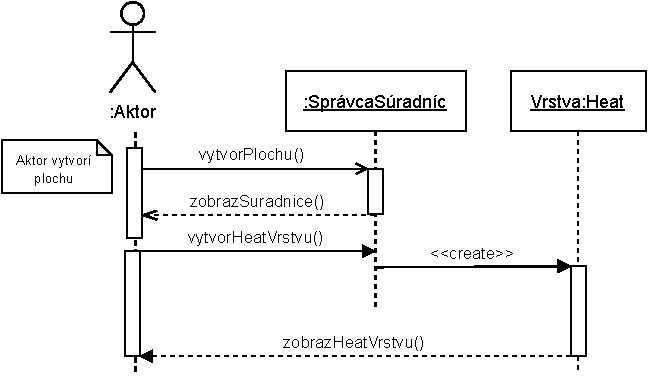
\includegraphics[width=0.9\linewidth]{obrazky-figures/seq-diagram.pdf}
    \caption{Sekvenčný diagram, ktorý zobrazuje, v akom poradí budú vykonávané jednotlivé operácie.}
    \label{fig:navrh-diagram}
\end{figure}

Aby systém fungoval správne, bude potrebné brať vstupné údaje o pravdepodobnostiach. Tieto pravdepodobnosti ale užívateľ nebude môcť zadať v užívateľskom grafickom rozhraní. Keďže každá značka má definované, aké môže mať kľúče s~hodnotami (\texttt{key=value}), bude potrebné pre~každú takúto dvojicu hodnôt priradiť hodnoty, ktoré budú vytvárať heat vrstvu. 


\section{Funkcionalita}
Analýzou požiadavkov sa podarilo navrhnúť systém, ktorý bude spĺňať tieto požiadavky. Primárnym cieľom je vytvoriť systém, ktorý bude zobrazovať mapu s~vytvorenou heat vrstvou zo~získaných dát.

\subsection*{Vytváranie oblasti}
Oblasť, z~ktorej bude chcieť zistiť odhad pravdepodobnosti osôb v danej oblasti, bude možné vybrať pomocou obdĺžnika, ktorý užívateľ nakreslí na~mapu. Z~vytvorenej oblasti budú následne použité hraničné súradnice daného nakresleného obdĺžnika na~vytvorenie dátového rámca s~geografickými objektami. 

\subsection*{Sťahovanie dát}
Získané hraničné súradnice sa použijú pri vytváraní heat vrstvy. Predtým by si systém mal stiahnuť dáta do~svojej pamäte. V~týchto dátach by mali byť uložené informácie o~geometrických objektoch, ktoré sa nachádzajú v~danej oblasti. Tieto informácie by mal systém získať pomocou požiadavku na~server alebo ich by mal mať uložené lokálne. Podľa~\cite{openstreet-stats} existuje vyše 86 tisíc rôznych kľúčov a~vyše 132 miliónov rôznych značiek na~celej mape sveta. Keďže na~vytvorenie heat vrstvy potrebujeme väčšinu značiek, pri takom veľkom množstve rôznych kľúčov by nebolo príliš efektívne sťahovať dáta z~webového rozhrania API. Preto je vhodnejšou alternatívou použitie lokálnych súborov, ktoré si bude užívateľ môcť stiahnuť a~vytvárať požiadavky na~tieto lokálne súbory.

\subsection*{Vytváranie heat vrstvy}
Vytvorená heat vrstva by mala byť súvislá u~všetkých geometrických objektoch. Nemala by nastať situácia, kedy časť geometrického objektu je pokrytá iba z~časti vrstvou heat mapy a~zvyšná časť je bez tejto vrstvy. Keďže geometrické objekty môžu byť jedným z~troch typov (bod, čiara alebo polygón), bude potrebné vyriešiť, ako sa bude zobrazovať heat vrstva pre jednotlivé geometrické objekty.

\textbf{Bod} môže na~mape predstavovať napríklad autobusovú zastávku. U~tohto typu je vykreslenie heat vrstvy najjednoduchšie zo~všetkých geometrických objektov, pretože budú stačiť dve hodnoty na~vykreslenie \--- zemepisná dĺžka a~zemepisná šírka daného bodu. Na~obrázku~\ref{fig:heat-point} je možné vidieť, ako by sa mala vykresliť heat vrstva pre určitý bod.

\begin{figure}[ht]
    \centering
    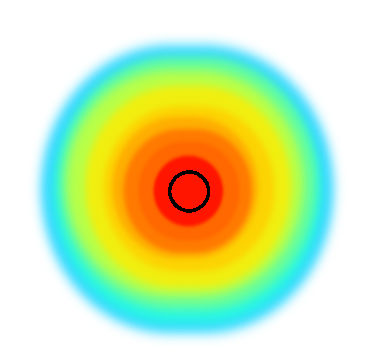
\includegraphics[width=0.3\linewidth]{obrazky-figures/heat-point.pdf}
    \caption{Heat vrstva na~geometrickom objekte typu bod.}
    \label{fig:heat-point}
\end{figure}

\textbf{Čiara} môže na~mape predstavovať napríklad cestu. Tento typ bude potrebné upraviť tak, aby heat vrstva na~danom geometrickom objekte bola súvislá. Na~obrázku~\ref{fig:heat-line} je možné vidieť, ako by mala vyzerať súvislá vykreslená heat vrstva pre čiaru.
 
 \begin{figure}[ht]
     \centering
     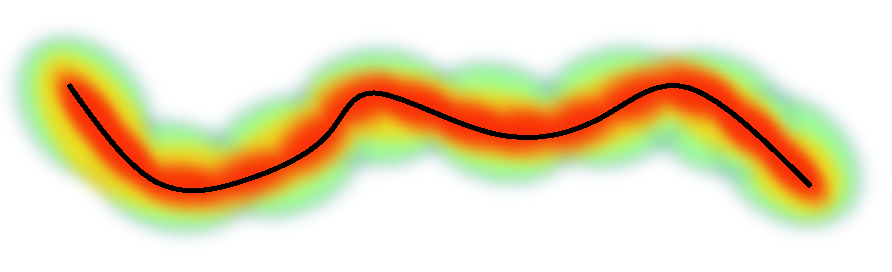
\includegraphics[width=0.8\linewidth]{obrazky-figures/heat-line.pdf}
     \caption{Heat vrstva na~geometrickom objekte typu čiara.}
     \label{fig:heat-line}
 \end{figure}
 
 \textbf{Polygón} môže na~mape predstavovať rôzne budovy, napríklad školu. Vnútro polygónu a~najbližšia oblasť okolo polygónu by mala byť v~červenej farbe. V~tejto oblasti by mala byť pravdepodobnosť výskytu osôb najvyššia. Postupne sa farba mení na studenšie farby a~vzniká tým súvislý prechod farieb ako u~bodu a~čiary. Na~obrázku~\ref{fig:heat-polygon} je možné vidieť, ako by mohla vyzerať heat vrstva pre polygón.
 
 \begin{figure}[ht]
     \centering
     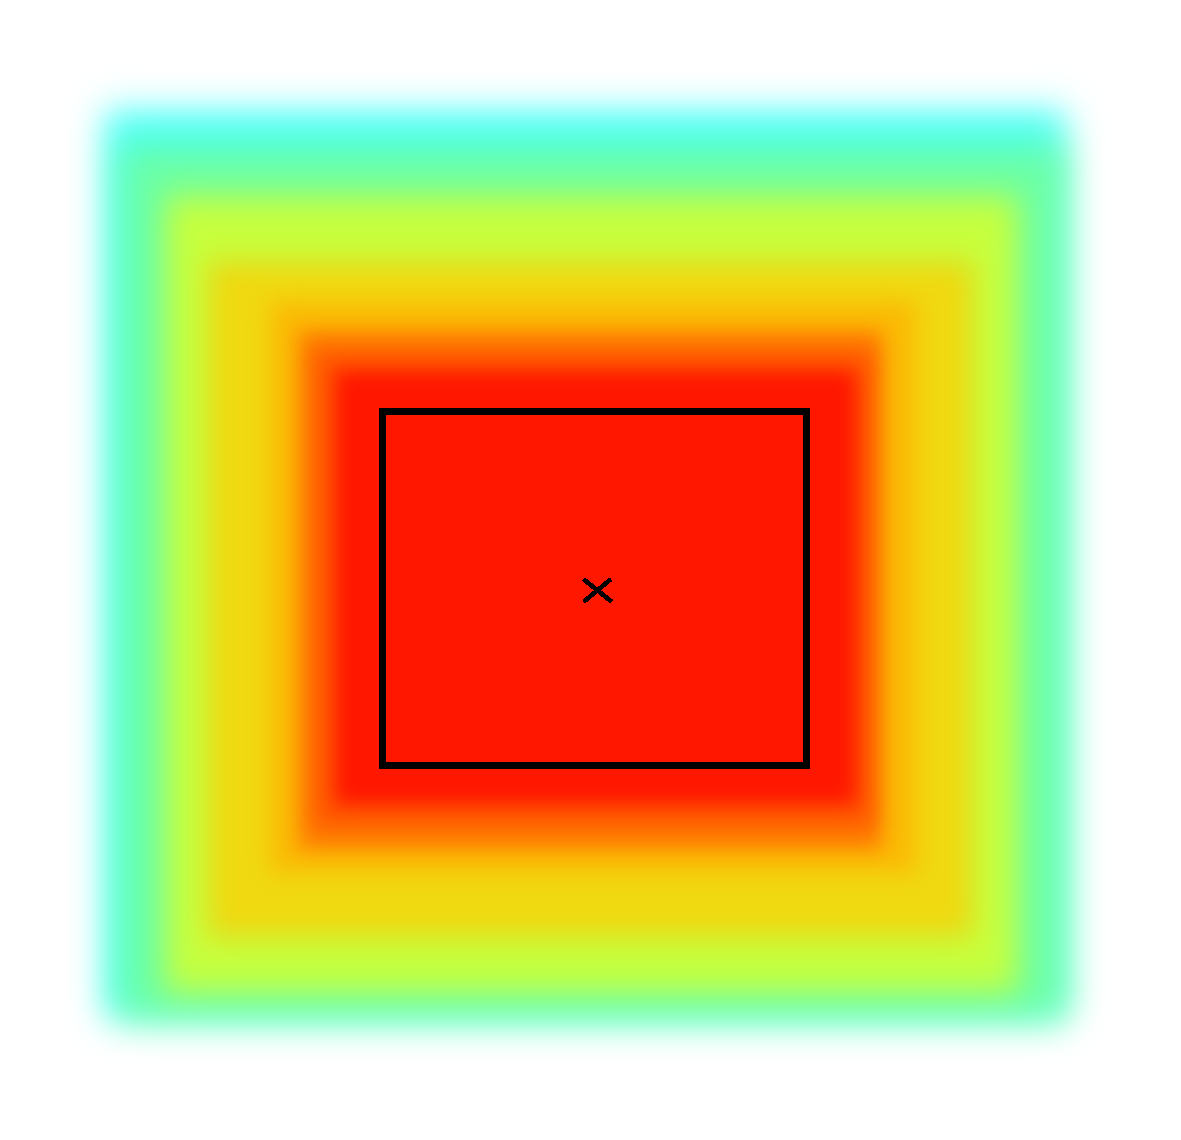
\includegraphics[width=0.5\linewidth]{obrazky-figures/heat-polygon.pdf}
     \caption{Heat vrstva na~geometrickom objekte typu polygón. Prechod vrstiev sa vyvíja od~stredového bodu polygónu, ktorý je vyznačený na~obrázku značkou \texttt{$\times$}.}
     \label{fig:heat-polygon}
 \end{figure}
 

\section{Návrh užívateľského rozhrania}
Hlavným cieľom užívateľského rozhrania bude umožnenie užívateľovi vytvoriť plochu, na~ktorej sa má vykresliť heat vrstva. Časť užívateľského rozhrania bude inšpirovaná užívateľským rozhraním stránky OpenStreetMap\footnote{\url{https://www.openstreetmap.org}}, a to získavanie vstupných súradníc. Na~obrázku~\ref{fig:ui-mockup} je zobrazený návrh užívateľského rozhrania. Na ľavom paneli bude užívateľ môcť zadávať vstupné súradnice, vytvárať plochu, na ktorej chce vykresliť heat vrstvu, upravovať veľkosť plochy pomocou vstupného formulára. Na ľavom paneli sa bude nachádzať aj tlačítko na~vytvorenie mapy s~heat vrstvou. Napravo od ľavého panela sa bude nachádzať mapa, na ktorej sa bude zobrazovať heat vrstva. Aké hodnoty pravdepodobností dané farby predstavujú, bude zobrazené na~škále v~pravom hornom rohu mapy.

\begin{figure}[ht]
    \centering
    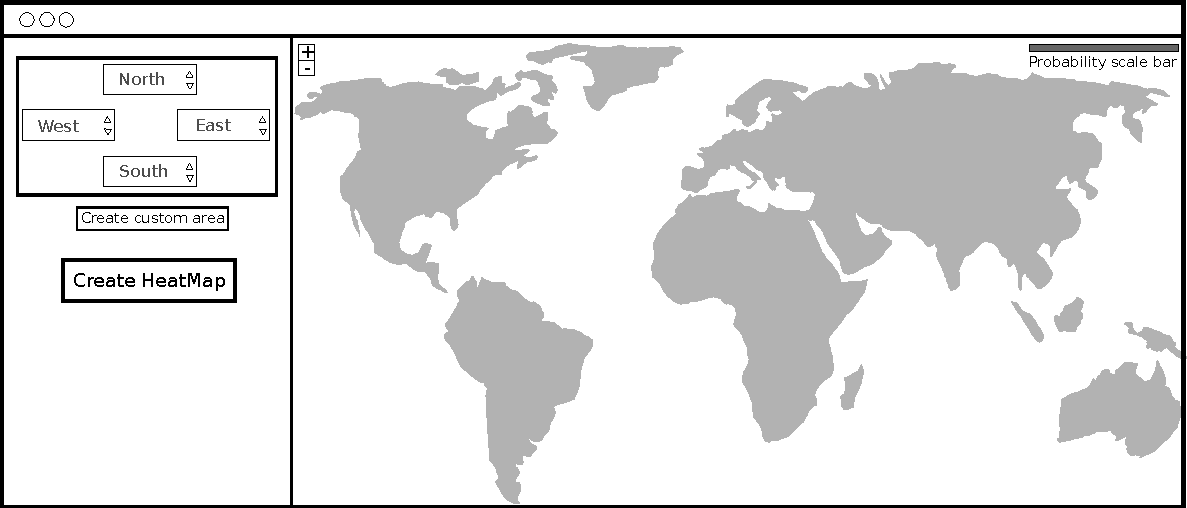
\includegraphics[width=0.98\linewidth]{obrazky-figures/ui-mockup.pdf}
    \caption{Návrh užívateľského rozhrania.}
    \label{fig:ui-mockup}
\end{figure}



\chapter{Implementácia}
\label{chap:implementacia}
V tejto kapitole je popísaná architektúra navrhnutej aplikácie, taktiež sú v tejto kapitole popísané použité technológie a~ako boli použité. Okrem toho je v~tejto kapitole popis implementácie funkcionality a~popis implementácie grafického užívateľského rozhrania.


\section{Architektúra}
Navrhnutá aplikácia rozširuje funkcionalitu projektu OpenStreetMap. Aplikácia pridáva do~projektu OpenStreetMap možnosť pridávania teplotnej vrstvy do zobrazenej mapy. Užívateľ si bude môcť vybrať oblasť mapy, pre ktorú by chcel zobraziť mapu s teplotnou vrstvou. Aplikácia teda nezobrazí vygenerovanú mapu s~teplotnou vrstvou pre celý svet naraz, ale iba pre časť mapy. Architektúra systému je založená na architektúre klient-server. Takýto typ architektúry umožňuje vytvoriť moduly, ktoré síce vykonávajú odlišné akcie, ale spoločne vytvárajú funkčný systém. Na~obrázku~\ref{fig:architecture} je možné vidieť, aké akcie vykonáva webový server a~aké akcie vykonáva klientská časť aplikácie.

\begin{figure}[ht]
    \centering
    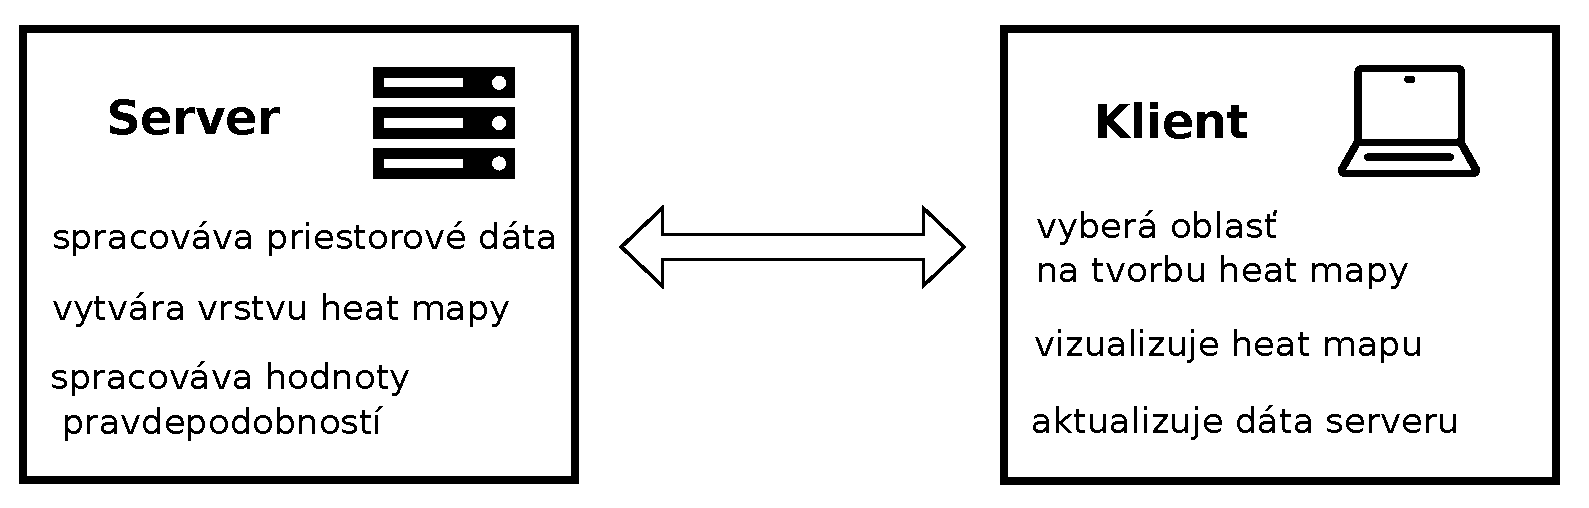
\includegraphics[width=0.95\linewidth]{obrazky-figures/architecture.pdf}
    \caption{Architektúra navrhovanej aplikácie.}
    \label{fig:architecture}
\end{figure}

Implementácia webového serveru je napísaná v~jazyku Python. Klientská časť aplikácie sa ukladá do~prehliadača užívateľa a~zobrazuje sa užívateľovi v~prehliadači, takže je zložená z~jazykov, ktoré slúžia pri vývoji webových aplikácií (Javascript, HTML a CSS). Obidve časti aplikácie si vzájomne vymieňajú informácie pomocou zvoleného webového frameworku. Okrem toho server má uložené informácie o~značkách a~ich pravdepodobnostiach, ktoré sa nachádzajú na~mape.


\section{Použité technológie}
Keďže aplikácia je navrhnutá ako klient-server aplikácia, je potrebné využiť vhodné technológie na~webovom serveri aj na~klientskej strane aplikácie. Funkcionalita danej aplikácie rozširuje pridávanie heat vrstvy do~mapy z~OpenStreetMap. Na strane servera je nutné spracovať priestorové dáta a~na~klientskej strane aplikácie zvoliť technológiu, ktorá by umožňovala zobrazovanie heat vrstvy na mape. Vytváranie aj takejto vrstvy na mapu umožňuje technológia \emph{Leaflet} a~jej rozšírenia vytvorené open-source komunitou. Aby si vedel užívateľ zobraziť danú vrstvu na mape, je potrebné zvoliť vhodnú technológiu, ktorá dokáže komunikovať s~klientskou stranou aplikácie. 


\section{Webový server}
Na webovom serveri prebieha spracovávanie priestorových dát a~ich spracovávanie na výstup. Okrem knižnice \emph{GeoPandas} v~programovacom jazyku Python neexistuje veľa technológií, ktoré by zjednodušovali spracovávanie priestorových dát. Keďže na~zobrazovanie dát na klientskej strane aplikácie je použitá knižnica Leaflet z jazyka Javascript, ktorý je používaný najmä pri tvorbe webových stránok, použitie webového frameworku je vhodnou voľbou. Okrem toho webové frameworky uľahčujú vytváranie webových aplikácií a~zobrazovanie spracovaných dát na~výstup.

\subsection*{Flask}
Flask\footnote{\url{https://flask.palletsprojects.com/en/2.1.x}} je mikro webový framework napísaný v programovacom jazyku Python. Flask nevyžaduje konkrétne nástroje ani ďalšie vnútorné knižnice. Aj keď sa tento framework považuje za mikro framework, neznamená to, že nie je možné ho rozširovať o rôzne služby~\cite{Oreilly2014Flask}.

Zobrazovať dáta vo webových aplikáciách je možné pomocou rôznych webových frameworkoch. Aplikácia je navrhnutá ako jednostránková aplikácia a~nevyžaduje vytváranie databázovej schémy. Na základe týchto vlastností som sa rozhodol nepoužiť webové frameworky, ktoré by boli príliš robustné na~použitie v~tejto aplikácii. Preto som sa rozhodol použiť webový framework Flask.

\subsection*{GeoPandas}
GeoPandas\footnote{\url{https://geopandas.org/en/stable}} je open-source projekt, ktorý umožňuje jednoduchú manipuláciu geografických dát v jazyku Python. Tento projekt je pokročilejší nástroj umožňujúci načítavanie GIS dát (.geojson, .gdb, .shp, \ldots), manipuláciu s GIS dátami, manipuláciu s~geometrickými útvarmi, prevádzanie súradnicových systémov a vykresľovanie máp. Základnými dátovými štruktúrami projektu GeoPandas sú \texttt{GeoDataFrame} a \texttt{GeoSeries}. Tieto dve dátové štruktúry sú nadstavbou knižnice \emph{Pandas}\footnote{\url{https://pandas.pydata.org}}, pretože rozširujú možnosti dátových štruktúr \texttt{Series} a \texttt{DataFrame} z tejto knižnice.

\texttt{GeoDataFrame} je dvojrozmerná dátová štruktúra, podobná tabuľke s riadkami a~stĺpcami a~je podtriedou \emph{pandas.DataFrame} s pridaným stĺpcom \texttt{geometry} (obrázok~\ref{fig:dataframes}).

\texttt{GeoSeries} je jednorozmerná dátová štruktúra, ktorá je podtriedou \emph{pandas.Series} a~umožňuje ukladať geometrické objekty \--- body, čiary, polygóny, prípadne ich násobné varianty. Predstavuje stĺpec geometry v dátovej štruktúre GeoDataFrame.

\begin{figure}[ht]
    \centering
    \subfloat[\centering \textbf{DataFrame}]{{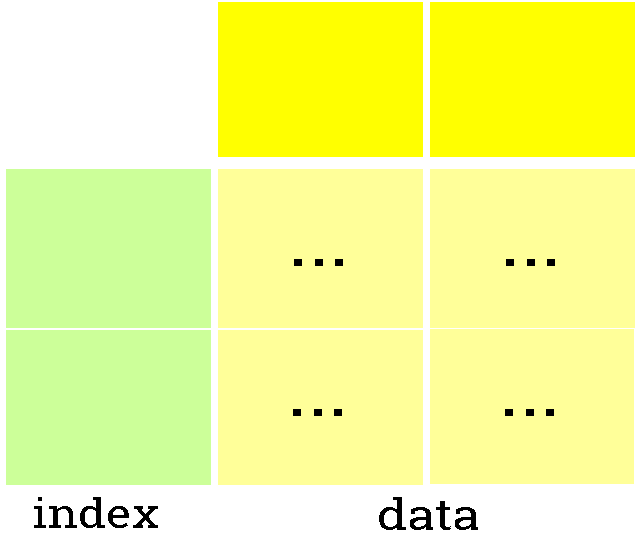
\includegraphics[width=0.25\linewidth]{obrazky-figures/dataframe.pdf}}}
    \qquad
    \subfloat[\centering \textbf{GeoDataFrame}]{{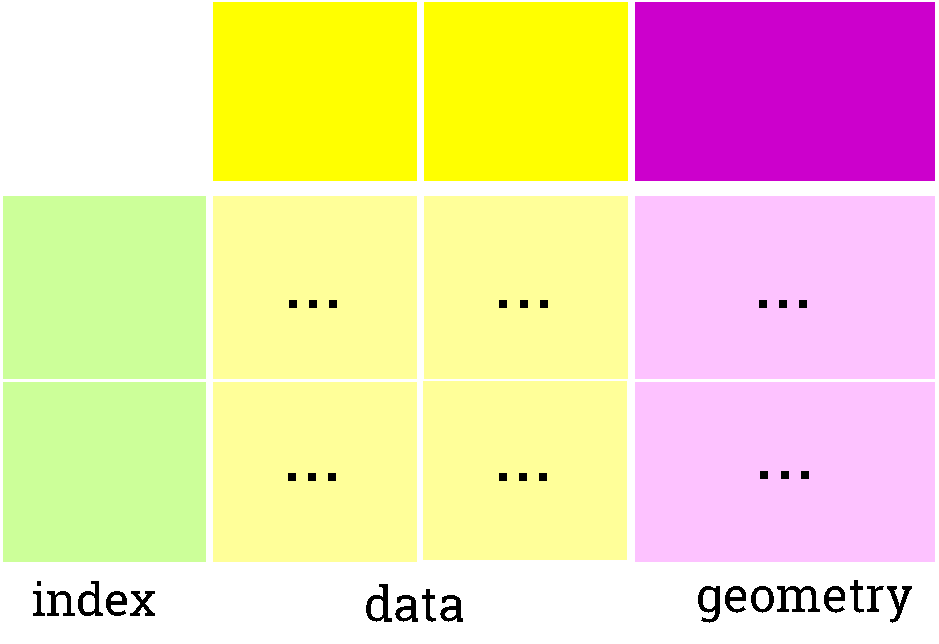
\includegraphics[width=0.31\linewidth]{obrazky-figures/geodataframe.pdf}}}
    \caption{Rozdiel medzi dátovými štruktúrami DataFrame a GeoDataFrame.}
    \label{fig:dataframes}
\end{figure}

Priestorové dáta bolo potrebné spracovať efektívnym spôsobom. V~programovacích jazykoch neexistuje veľa overených technológií, ktoré by podporovali prácu s~priestorovými dátami. Možnou alternatívou je použitie GIS softvérov, ktoré ale nie všetky sú zadarmo. Preto som sa na základe tohto rozhodol použiť programovací jazyk Python s~importovanou knižnicou GeoPandas, ktorá umožňuje spracovávanie priestorových dát.

\subsection*{Ostatné nástroje}
Okrem ukladania dát do dátových rámcov je potrebné ich aj~upraviť do~formy, v~ktorej by sa dali použiť pri zobrazovaní heat vrstvy na~strane klienta. Medzi vhodné nástroje, ktoré umožňujú takúto úpravu dát v~jazyku Python, patria balíky nástrojov \emph{PyProj} a \emph{Shapely}.

\textbf{PyProj}\footnote{\url{https://pyproj4.github.io/pyproj/stable}} je rozhranie v~jazyku Python na PROJ\footnote{\url{https://proj.org}}. PROJ je softvér, ktorý sa používa na~transformovanie geografických súradníc z~jedného súradnicového systému do~iného súradnicového systému.

\textbf{Shapely}\footnote{\url{https://shapely.readthedocs.io/en/stable}} je balík nástrojov v~jazyku Python na~manipuláciu a analýzu rovinných geometrických objektov. Tento balík je vhodné použiť s~už zmieneným nástrojom PyProj, pretože Shapely sa nezaoberá tým, v~akom súradnicovom systéme je upravovaný geometrický objekt. 

Možnosť transformácie súradnicového systému na iný súradnicový systém bol využitý aj~pri implementácii aplikácie. U~niektorých geometrických útvaroch (konkrétne u čiar) bolo potrebné zistiť, aké sú hodnoty daného geografického objektu v inom súradnicovom systéme. Implicitne sú dátové rámce s~dátami o~geografických objektoch v~geografickom súradnicovom systéme (EPSG:4326), ktorý využíva uhlové jednotky. Takáto projekcia neumožňuje rôzne úpravy takýchto geometrických objektov. Transformovaním na~projektovaný súradnicový systém (EPSG:3857) je možné dostať vzdialenosti bodov na~mape v~metroch.


\section{Klientská časť}
\addtocontents{toc}{\protect\setcounter{tocdepth}{1}}
Na klientskej časti aplikácie vyberá užívateľ oblasť, na~ktorej sa má vytvoriť heat vrstva. Keď užívateľ vyberie oblasť, pošle sa požiadavka na server, na~ktorom sa spracujú zadané vstupné hodnoty a~odošlú sa dáta na~tvorbu heat vrstvy späť klientovi.

Existuje veľa knižníc, ktoré umožňujú vytvárať heat grafy resp. heat vrstvy. Vytváranie heat vrstiev je možné aj v~jazyku Python pomocou knižnice \emph{Seaborn}\footnote{\url{https://seaborn.pydata.org/generated/seaborn.heatmap.html}}, ale táto knižnica neumožňuje zobrazovanie heat vrstvy spoločne už so~zobrazenou mapou. Takisto prechod medzi jednotlivými farbami nie je plynulý. Keďže heat vrstvy sa majú vytvárať na klientskej časti aplikácie, je potrebné použiť nástroje jazykov, ktoré sa používajú na strane klienta. Preto som sa rozhodol použiť knižnicu \emph{Leaflet} implementovanú v jazyku Javascript.

\subsection{Leaflet}
Leaflet\footnote{\url{https://leafletjs.com}} je open-source knižnica v programovacom jazyku JavaScript, používaná na vytváranie mapových webových aplikácii. Táto knižnica je podporovaná na väčšine mobilných a desktopových zariadeniach. Leaflet umožňuje vývojárom jednoducho zobrazovať webové mapy s dlaždicami, získavať geopriestorové dáta zo súborov typu GeoJSON, vytvárať interaktívne vrstvy a~pod.

Okrem základnej funkcionality existujú rôzne rozšírenia, ktoré rozširujú základnú funkcionalitu knižnice Leaflet. V mojej aplikácii sa používajú dve rozšírenia k tejto knižnici: \texttt{Leaflet.heat} a~\texttt{Leaflet.draw}.

\subsubsection{Rozšírenie Leaflet.heat}
Základom tejto knižnice je knižnica \texttt{simpleheat} z jazyka JavaScript, ktorá sa používa na~kreslenie heat máp na plátno. Na vytvorenie vrstvy heat vrstvy na~mapu sa používa funkcia \texttt{L.heatLayer(latlngs, options)}, kde:
\begin{itemize}
    \item \texttt{latlngs} \--- predstavuje dvojrozmerné pole, kde každé pole v tomto poli je definované dvojicou (zemepisná dĺžka, zemepisná šírka) resp. trojicou hodnôt (zemepisná dĺžka, zemepisná šírka, intenzita),
    \item \texttt{options} \--- má viacero možnosti, ktoré sa dajú zadefinovať pre danú vrstvu, najdôležitejšie z nich pre moju aplikáciu sú:
    \begin{itemize}
        \item \texttt{max} \--- maximálna intenzita bodu, implicitná hodnota je 1.0,
        \item \texttt{radius} \--- rádius každého bodu na heat mape, implicitná hodnota je 25,
        \item \texttt{blur} \--- množstvo rozptýlenia, implicitná hodnota je 15,
        \item \texttt{gradient} \--- konfigurácia prechodu farieb.
    \end{itemize}
\end{itemize}

Na~obrázku~\ref{fig:leafletheat} je možné vidieť ako sa dá pridať heat vrstva do~mapy a~ako daná vrstva vyzerá na~mape. Hodnoty intenzít, ktoré sú treťou hodnotou každého vykresleného bodu, udávajú hodnotu pravdepodobnosti pre danú značku na~mape. To znamená, že ak ide napríklad o~školu, na~mape sa vykreslí bod pre danú značku s~intenzitou~$1.0$. Na druhú stranu, ak by išlo o~značku, ktorá by značila lesnú cestu, intenzita farby pre danú značku by bola nižšia.

\lstset{
    caption={},
    label={},
    basicstyle=\ttfamily\footnotesize\bfseries
}
\begin{figure}[ht]
\begin{minipage}{.5\textwidth}
\begin{lstlisting}
var heat = L.heatLayer([
     // lat, lng, intensity
    [49.1784, 16.7772, 0.2],
    [49.1784, 16.7774, 0.4],
    [49.1784, 16.7776, 0.6],
    [49.1784, 16.7778, 0.8],
    [49.1784, 16.7780, 1.0]
], {radius: 30}).addTo(map);
\end{lstlisting}
\end{minipage}
\hfill
\begin{minipage}{.5\linewidth}
    \centering
    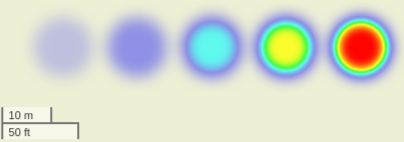
\includegraphics[width=0.7\linewidth]{obrazky-figures/heatlayer-screenshot.png}
\end{minipage}
\caption{\textbf{Rozšírenie Leaflet.heat}. Vľavo sa nachádza implementácia vrstvy, zoradená vzostupne podľa hodnôt intenzít, vpravo sa nachádza zobrazenie týchto bodov na~mape.}
\label{fig:leafletheat}
\end{figure}

\subsubsection{Rozšírenie Leaflet.draw}
Na to, aby užívateľ mohol vybrať určitú oblasť z mapy, na ktorej sa má vykresliť heat vrstva, bolo potrebné použiť rozšírenie Leaflet.draw. Ako je možné vidieť na~obrázku~\ref{fig:leafletdraw}, na bočnom paneli mapy v hornom ľavom rohu sa nachádza panel nástrojov, ktorý umožňuje kresliť geometrické útvary na mapu a následne ich upravovať alebo aj vymazávať. Pre~jednoduchosť aplikácie na vybratie určitej oblasti pomocou geometrických tvarov bol použitý iba jeden geometrický tvar \--- obdĺžnik.

\begin{figure}[ht]
    \centering
    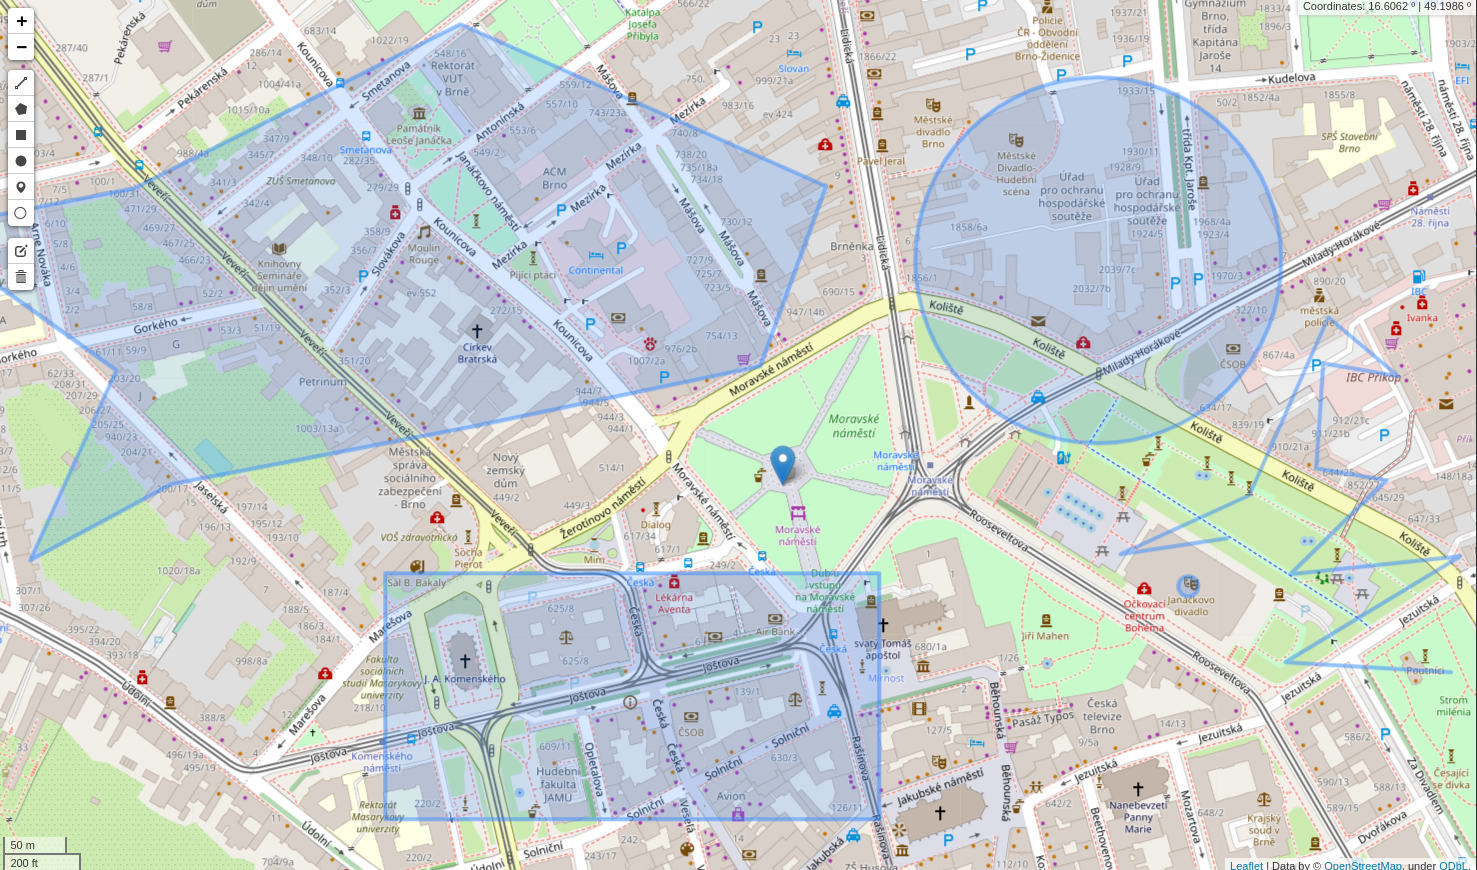
\includegraphics[width=0.9\textwidth]{obrazky-figures/leaflet-draw-screenshot.png}
    \caption{\textbf{Rozšírenie Leaflet.draw} pridáva možnosť kreslenia geometrických útvarov na~mapu \-- krivky, polygóny, obdĺžniky, kruhy, značky a~kruhové značky. Okrem toho je možné pomocou tohto rozšírenia upravovať, presúvať a vymazávať geometrické útvary.}
    \label{fig:leafletdraw}
\end{figure}

\subsection{HTML}
Jazyk HTML\footnote{HyperText Markup Language, v preklade \emph{Hypertextový značkovací jazyk}.} je jazyk určený na vytváranie webových stránok. Ako už názov napovedá, slovo \emph{hypertextový} naznačuje možnosť odkazov jednotlivých stránok na ostatné. Slovo \emph{značkovací} v spojitosti s jazykmi predstavuje jazyky, ktoré doplňujú text o tzv. \emph{značky} resp.~\emph{tagy}. Všetky značky majú svoje atribúty, ktoré upresňujú jej parametre. Jednotlivé značky je možné do seba vnárať a~spolu tak vytvárajú hierarchickú štruktúru~\cite{kosek1998html}.

\subsection{CSS}
Štruktúru webových stránok je možné vytvoriť použitím len jazyka HTML, ale na to, aby stránky vyzerali užívateľsky prívetivo, je nutné použiť aj iné nástroje, ktoré pôsobia na~užívateľa prívetivejším dojmom. Preto vznikol mechanizmus \emph{CSS}\footnotetext{Cascading Style Sheets} na vizuálne formátovanie webových stránok. Tento mechanizmus slúži na popis kaskádových štýlov HTML dokumentu.

\subsection{JQuery}
JQuery\footnote{\url{https://jquery.com}} je rýchla a cross-browser\footnote{Cross-browser kompatibilita je schopnosť webových stránok fungovať v rôznych prehliadačoch.} knižnica z jazyka JavaScript. Zjednodušuje prechádzanie dokumentov HTML, výber DOM\footnote{Document Object Model} elementov, kontrolu udalostí alebo aj vytváranie animácií. Výhodou tejto knižnice je, že je jednoduchou knižnicou na vývoj webových aplikácií. Oproti iným knižniciam v JavaScripte nevyžaduje lepšiu skúsenosť s jazykom JavaScript. Táto knižnica umožňuje okrem už zmienených možností, jednoduchšiu obsluhu \texttt{AJAX} volaní.

\subsection{AJAX}
Technológia AJAX\footnote{Asynchronous JavaScript and XML} umožňuje meniť obsah stránok bez potreby kompletného načítania zo~servera. Keďže protokol HTTP je bezstavový, akékoľvek stavové informácie je nutné posielať pri každej požiadavke servera a~opačne. AJAX nám umožňuje sa takémuto postupu vyhnúť~\cite{lacko2008ajax}. Ako je možné poznať z názvu, AJAX je kombinácia viacerých prvkov:
\begin{itemize}
    \item HTML a CSS na prezentovanie informácií,
    \item DOM na zobrazenie prezentovaných informácií,
    \item metóda na výmenu dát medzi prehliadačom a serverom (napr. XMLHttpRequest objekt),
    \item formát dát posielaný medzi prehliadačom a serverom (napr. XML)
\end{itemize}

V mojej aplikácií som použil AJAX technológiu na aktualizáciu súradníc pri zmene veľkosti alebo presune oblasti určenej na vytvorenie heat mapy.

\subsection{Bootstrap}
Bootstrap je sada nástrojov, ktorá obsahuje rozšírenie pre jazyky HTML, CSS a JavaScript. Umožňuje vytvárať pomocou veľkého množstva rôznorodých komponentov interaktívne webové stránky. Vyžaduje určitú znalosť HTML a~CSS, pretože väčšinu komponentov je možné vkladať iba pomocou HTML a CSS~\cite{bootstrap}.

V mojej aplikácií používam tzv. \emph{Alert} komponentu t.j. výstražnú správu. Ak sa nepodarila vytvoriť heat mapa z~parametrov poslaných na server, server pošle správu užívateľovi, že heat mapa sa pre zadanú oblasť nepodarila vytvoriť.


\section{Implementácia funkcionality}
Implementácia funkcionality vychádza z~návrhu, ktorá bola popísaná v~kapitole~\ref{chap:navrh}. Ako implementačný programovací jazyk bol vybratý Python spolu s~knižnicami, ktoré boli popísané v~tejto kapitole. Pri vytváraní heat vrstvy je potrebné urobiť viacero úprav dát, aby sa v~aplikácii zobrazovali relevantné dáta na~mape.

\subsection*{Spracovanie hodnôt pravdepodobností}
Prvou potrebnou vecou, ktorú systém spracováva, sú dáta pravdepodobností pre jednotlivé značky. Dáta o~značkách sú uložené v~súbore, ktorý je vo~formáte JSON. Tieto dáta sú prednastavené s~tým, že tieto hodnoty užívateľ môže pozmeniť v~tomto súbore, prípadne pridať alebo odstrániť niektoré hodnoty. Súbor sa v~systéme spracuje a~uloží sa ako asociatívne pole do~pamäte, s~ktorým bude systém pracovať pri úprave dátového rámca.

\subsection*{Vytvorenie dátového rámca}
Keďže pri vyššom počte hodnôt pravdepodobností pre jednotlivé značky by počet požiadaviek na webové rozhranie API bol vysoký, systém spracováva požiadavky z~lokálnych súborov. Tieto súbory sú vo~formáte \emph{shapefile} a~sú získané zo~stránky Geofabrik\footnote{\url{https://download.geofabrik.de}}. Súbory sú pomenované podľa názvu kľúča, ktorý sa nachádza v~danom súbore. Keďže súbory tohto formátu sú naviazané medzi sebou, pri spracovávaní týchto súborov nám stačí súbor vo~formáte \texttt{*.shp}, z~ktorého je možné vytvoriť dátový rámec so~stĺpcom o~geografických objektoch.

Vytvorený dátový rámec má viacero stĺpcov, ale využiteľné pre tento systém je iba stĺpec s~typom značky a~stĺpec s~geometrickými objektami. Každý riadok v~tomto rámci predstavuje jeden geometrický objekt na~mape. Ak sa daná značka pre daný geometrický objekt nenachádza vo~vytvorenom asociatívnom poli s~pravdepodobnosťami pre značky, riadok s~touto značkou sa preskočí.

\subsection*{Úprava geometrických objektov}
Každý riadok v~dátovom rámci sa spracuje podľa toho, aký predstavuje geometrický objekt. Jednotlivé riadky v~dátovom rámci je potrebné upraviť do~zoznamu bodov, ktorý sa použije pri vytváraní heat vrstvy pomocou knižnice \texttt{Leaflet.heat}. Vytvorením zoznamu bodov vznikne iba jedna súvislá heat vrstva, ktorá je vhodnejšia pri zobrazovaní na~mape.

\textbf{Bod} predstavuje jednoduchý geometrický objekt na~mape, pretože je reprezentovaný iba dvoma hodnotami \--- zemepisnou dĺžkou a~zemepisnou šírkou. K~týmto dvom hodnotám sa pridá tretia hodnota, ktorá pridáva intenzitu k~danému bodu.

\textbf{Čiara} je geometrický objekt na~mape, ktorý slúži na~zobrazovanie ciest. Heat vrstva pre cesty bez zákrut by sa bez dodatočnej úpravy vykreslili iba s~dvoma bodmi \--- počiatočným bodom a~koncovým bodom cesty. Takéto riešenie nie je vhodné, preto je lepším riešením takéhoto problému použiť interpoláciu úsečky. Na interpoláciu úsečky je použitá rovnica~\ref{eq:interpolate} odvodená z~obrázka~\ref{fig:interpolate}:

\begin{equation}
    y = y_1 + \frac{(x - x_1)(y_2 - y_1)}{x_2 - x_1},
    \label{eq:interpolate}
\end{equation}
kde $x_1$ a $y_1$ sú prvé súradnice, $x_2$ a $y_2$ sú druhé súradnice, $x$ je stredná hodnota hodnôt $x_1$ a $x_2$, a $y$ je hľadaná interpolovaná hodnota. Koľkokrát interpolujeme danú úsečku závisí od~dĺžky danej úsečky.

\begin{figure}[ht]
    \centering
    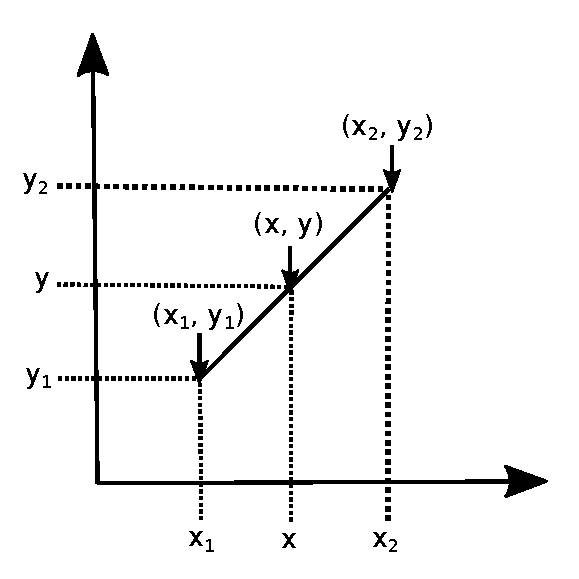
\includegraphics[width=0.4\linewidth]{obrazky-figures/linear-interpolation.pdf}
    \caption{Interpolácia úsečky.}
    \label{fig:interpolate}
\end{figure}

\textbf{Polygón} je geometrický objekt na~mape, ktorý slúži na zobrazovanie budov. Z~polygónov sa dajú získať iba okrajové body, body vo~vnútrajšku polygónov je potrebné zistiť pomocou vhodnej metódy. Najjednoduchším spôsobom, ktorý som použil aj~pri implementácii, je získanie stredového bodu polygónu. Na~obrázku~\ref{fig:polygon-center} je zobrazený zistený stredový bod pre rôzne typy obdĺžnikov. Na~zistenie stredového bodu polygónu bola použitá funkcia \texttt{centroid} z~knižnice GeoPandas.

\begin{figure}[ht]
    \centering
    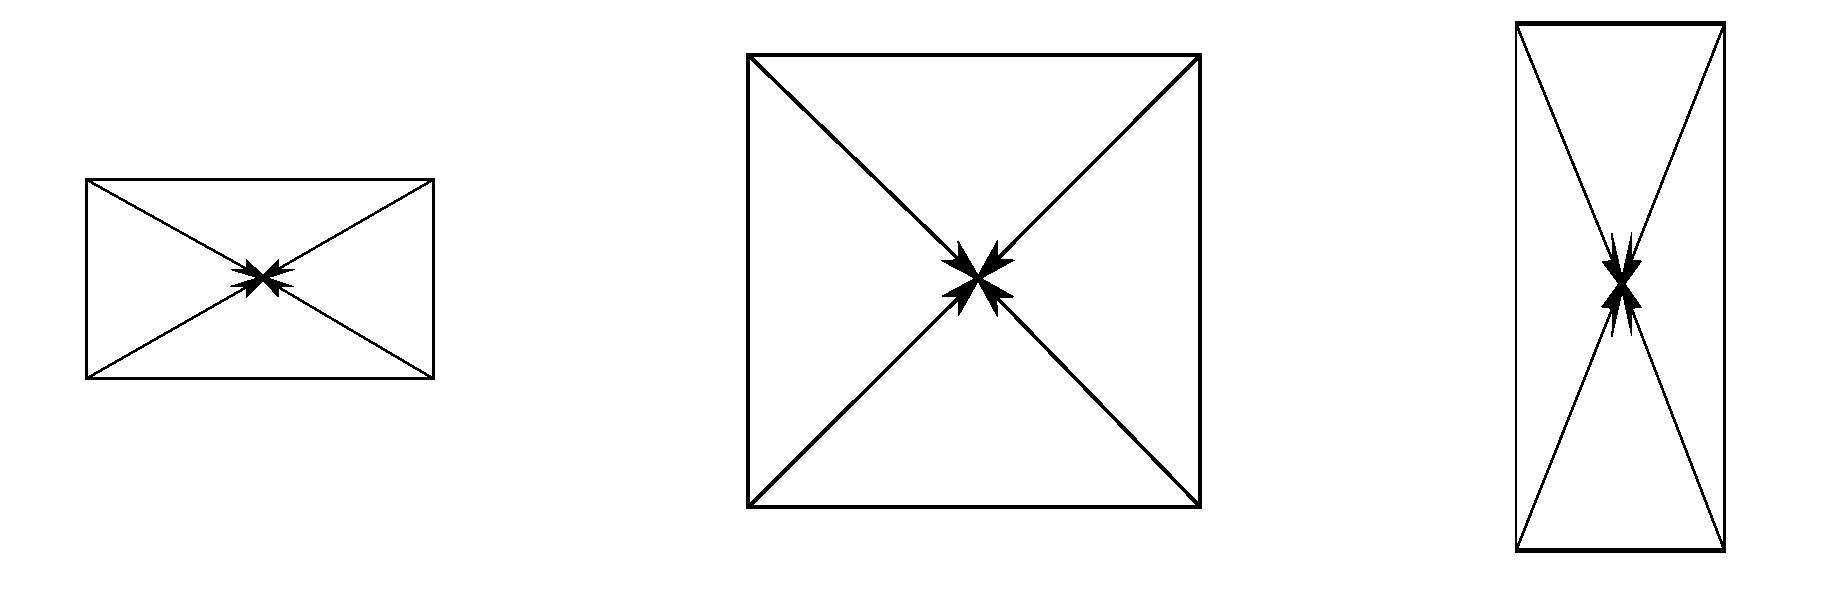
\includegraphics[width=0.8\linewidth]{obrazky-figures/polygon-center.pdf}
    \caption{Zistenie stredového bodu pre rôzne typy polygónov.}
    \label{fig:polygon-center}
\end{figure}

\subsection*{Vytvorenie heat vrstvy}
Po upráve geometrických objektov na~body a~následné vytvorenie zoznamu z~týchto bodov je možné vytvoriť heat vrstvu na~mape. Pri vytváraní heat vrstva sa zapisuje vytvorený list bodov do~súboru HTML. Tento súbor je poslaný klientovi do~prehliadača po~dokončení požiadavky.


\section{Implementácia užívateľského rozhrania}
Užívateľské rozhranie sa skladá z~viacerých komponentov, ktoré vytvárajú jednotný celok. V~ľavom paneli sa nachádza panel, v~ktorom môže užívateľ zadávať vstupné súradnice a~upravovať ich. V hlavnej časti obrazovky sa nachádza zobrazená mapa, na~ktorú sa vykresľuje heat vrstva. Na~zobrazenej mape sa nachádza aj~škála pre vytvorenú heat vrstvu. 

\subsection*{Získavanie vstupných súradníc}
Vstupné súradnice, ktoré zadal užívateľ, je potrebné aktualizovať pri každom zmenšení alebo zväčšení mapy resp.~oblasti vytvorenej pomocou nástroja \texttt{Leaflet.draw}. Pri nakreslení oblasti sa pomocou nástroja AJAX, ktorý bez potreby kompletného načítania stránky zo~servera, upravia súradnice vo~formulári na~ľavom paneli aplikácie. AJAX správa sa pošle po vytvorení oblasti na~mape pomocou udalosti \texttt{L.Draw.Event.CREATED} a~spustí sa udalosť \texttt{L.Draw.Event.EDITSTART}. Táto udalosť umožní užívateľovi meniť veľkosť aj~polohu nakreslenej oblasti. Odkaz na~vytvorenie oblasti (\texttt{Create custom area}) sa po tejto udalosti zmení na odkaz na~vymazanie vytvorenej oblasti (\texttt{Delete custom area}).

\subsection*{Škála pravdepodobností}
Zo~získaných hodnôt pravdepodobností pre každú značku je možné vytvoriť škálu, ktorá ukazuje, aká je odhad pravdepodobnosti osôb v~danej oblasti. Na~vytvorenie tejto škály bol použitý nástroj \emph{D3.js\footnote{\url{https://d3js.org}}}. Keďže funkcia \texttt{Leaflet.heatLayer()} umožňuje pridávať vlastne vytvorenú konfiguráciu prechodu farieb, táto škála je prepojená s~vytvorenou heat vrstvou. Aby sa zjednodušilo vytváranie takejto škály, na vytvorenie tejto farebnej škály bol použitý nástroj \emph{branca\footnote{\url{https://python-visualization.github.io/branca}}}, konkrétne modul pre prácu s~farebnými mapami. Vo~výslednej implementácii tejto aplikácie sa tento nástroj nepoužíva.



\chapter{Vyhodnotenie výsledkov}
\label{chap:vyhodnotenie}
Táto kapitola sa zaoberá ovládaním, testovaním a~vyhodnotením výsledkov z~vytvorenej aplikácie. V~tejto kapitole sa nachádza aj~popis možných chyby a~nevýhody implementovaného systému. Okrem toho, táto kapitola popisuje ako by sa dali vylepšiť získané dáta.


\section{Ovládanie}
Keďže aplikácia má slúžiť primárne pri plánovaní výstavby elektroenergetických zariadení na~území Českej republiky, pri ovládaní aplikácie je potrebné vybrať oblasť, ktorá sa nachádza na~území Českej republiky. Užívateľ si prípadne môže stiahnuť mapové dáta aj~pre iné krajiny na~svete. Z~užívateľského hľadiska je aplikáciu jednoduché ovládať, pretože neobsahuje veľa možností, ktoré užívateľ môže vykonať. Na~obrázku~\ref{fig:bosovice-map} je snímok obrazovky časti mapy s~nakresleným obdĺžnikom, kde sa nachádza obec Bošovice. Hraničné body tohto obdĺžnika sa použijú pri získavaní geografických dát. Veľkosť aj~polohu tohto obdĺžnika môže užívateľ ľubovoľne meniť.

\begin{figure}[ht]
    \centering
    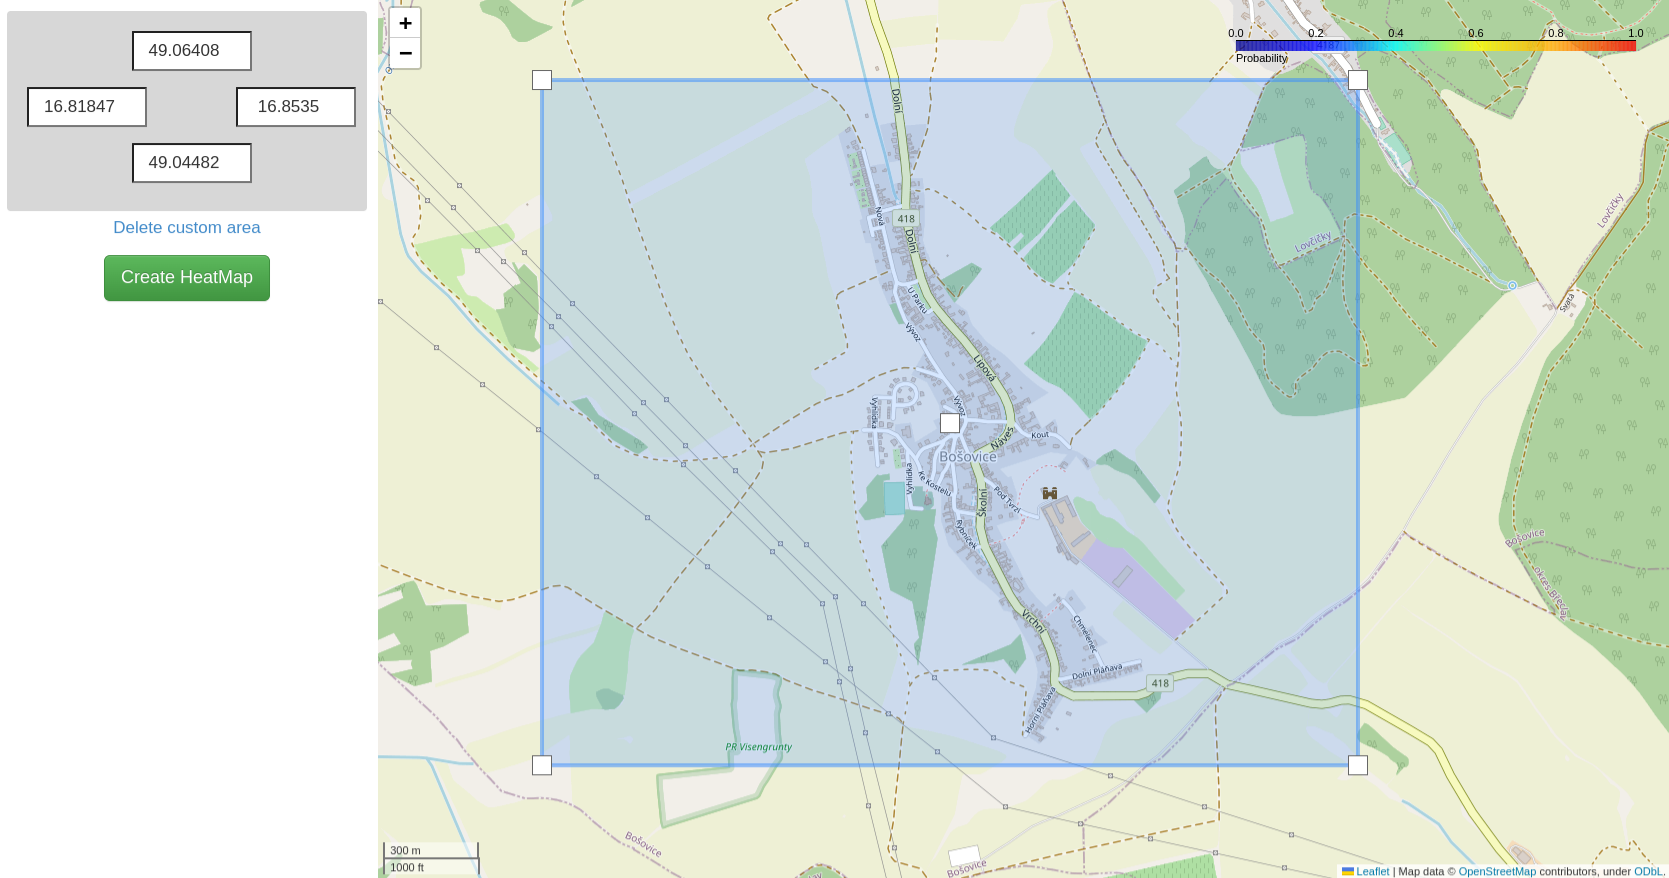
\includegraphics[width=1.0\linewidth]{obrazky-figures/bosovice-map.png}
    \caption{Výber oblasti na~mape.}
    \label{fig:bosovice-map}
\end{figure}

Po stlačení tlačítka \texttt{Create HeatMap} sa vytvoria zo~vstupných súborov dátové rámce. Následne sa k~nim pripoja hodnoty pravdepodobností a~vytvorí sa z~týchto bodov výstupná heat vrstva, ktorá sa zobrazí na mape. Na~obrázku~\ref{fig:bosovice-heatmap} je možné vidieť, ako vyzerá vytvorená heat vrstva na~mape. Táto vrstva sa zobrazí aj~mimo vybranej oblasti. Je to z~dôvodu, že geografické objekty typu cesta a~polygón sú tvorené viacerými bodmi. Niektoré z~týchto geografických objektov môžu sčasti presahovať vybranú oblasť. Aby sa zbytočne nevytvárali náročné výpočty v~aplikácii, berie sa celá plocha geometrických objektov, ktoré sa nachádzajú aspoň sčasti vo~vybranej oblasti.

\begin{figure}[ht]
    \centering
    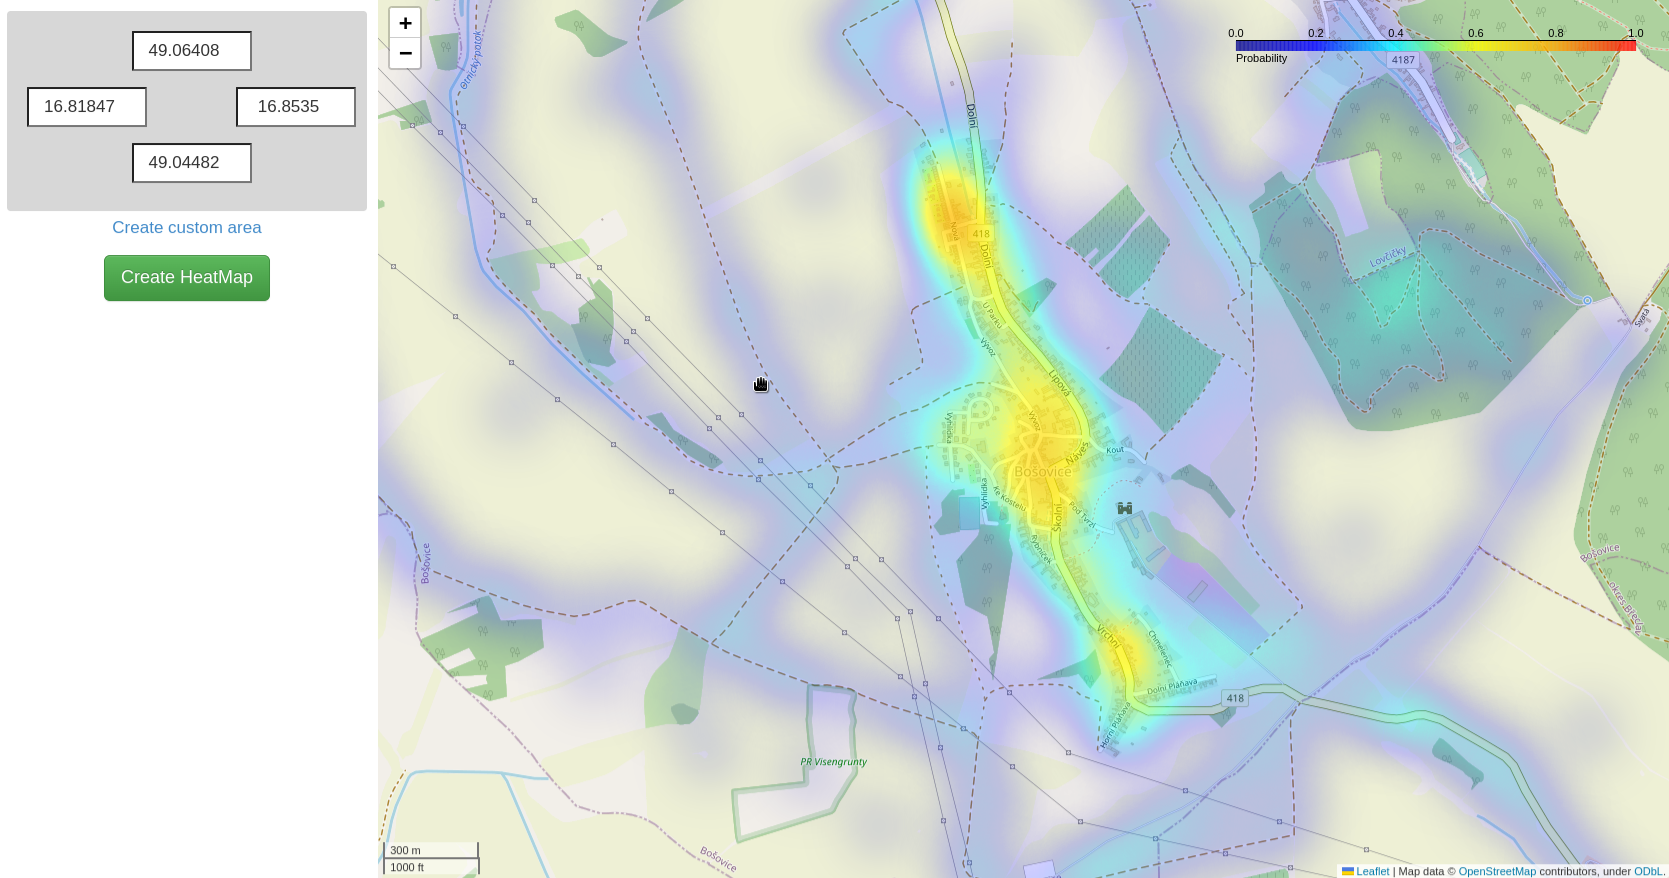
\includegraphics[width=1.0\linewidth]{obrazky-figures/bosovice-heatmap.png}
    \caption{Heat vrstva pre vybranú oblasť.}
    \label{fig:bosovice-heatmap}
\end{figure}


\section{Testovanie aplikácie}
Pri prvotnej implementácii sa brali mapové dáta pomocou API požiadavkov na~server. Takáto implementácia vytvorila veľa požiadavkov na~daný server a~viedlo to k~tomu, že by sa pri väčšom počte značiek v~danej oblasti muselo sťahovať veľké množstvo dát. To viedlo k~spomaleniu aplikácie. Preto vhodnejšou alternatívou, ktorá bola použitá, bolo stiahnutie dát z~webového serveru pred spustením aplikácie. Získanie lokálnych dát viedlo k~výraznému zrýchleniu aplikácie a~vylepšeniu samotnej implementácie aplikácie.

Hlavným výstupom aplikácie je mapa s~vytvorenými heat vrstvami. Na obrázku~\ref{fig:output-heat} je možné vidieť dva rôzne výstupy aplikácie. Ľavý obrázok predstavuje oblasť v~časti Brno-Medlánky, v ktorej sa nachádzajú chaty. V~tejto oblasti je heat vrstva zobrazená iba nad chatami, okolité oblasti sú bez takejto vrstvy. Pravý obrázok predstavuje zastavanú oblasť, konkrétne o~obec Nuzířov resp. ide o~časť obce Malhostovice v~okrese Brno-venkov v~Juhomoravskom kraji. Tento obrázok ukazuje, že najväčšia pravdepodobnosť odhadu výskytu osôb v~tejto obci je v~strednej časti obce.

\begin{figure}
    \centering
    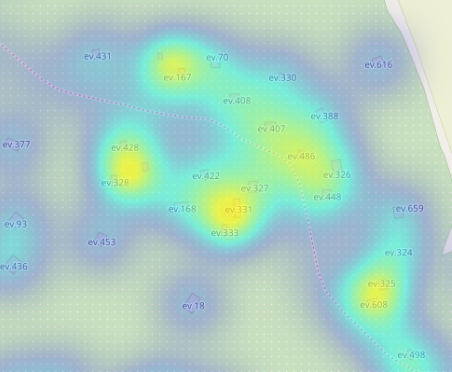
\includegraphics[width=0.48\linewidth]{obrazky-figures/brno-medlanky.png}\hfill
    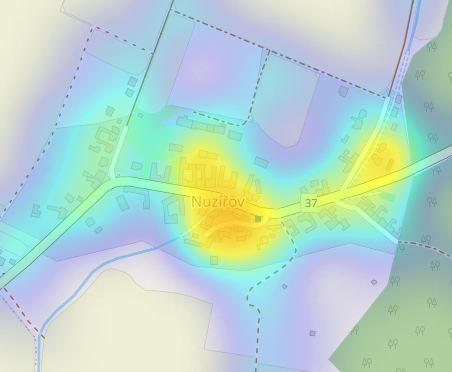
\includegraphics[width=0.48\linewidth]{obrazky-figures/nuzirov.png}
    \caption{Heat vrstva dvoch rôznych oblastí mapy.}
    \label{fig:output-heat}
\end{figure}


\section{Obmedzenia aplikácie}
Odhad pravdepodobnosti v~danej oblasti je iba teoretický, pretože aplikácia zatiaľ neberie do~úvahy viacero aspektov. Všetky aspekty nie je možné implementovať triviálne, pretože nie všetky sa dajú vyriešiť nástrojmi, ktoré existujú v~programovacích jazykoch.

\textbf{Zastavané oblasti v~obciach} by mali byť tiež pokryté heat vrstvou. Na~obrázku~\ref{fig:brno-zastavana-oblast} je možné vidieť, že časti zastavaných oblastí sú bez vytvorenej heat vrstvy. Možným riešením daného problému by bolo použitie rastrovej siete v~danej oblasti, v~ktorej by sa zistili body vo vnútri tejto zastavanej plochy. Týmto by sa vytvorili body v~danej oblasti a~bolo by možné vytvoriť pomocou toho súvislú heat vrstvu na~danej mape.

\begin{figure}[ht]
    \centering
    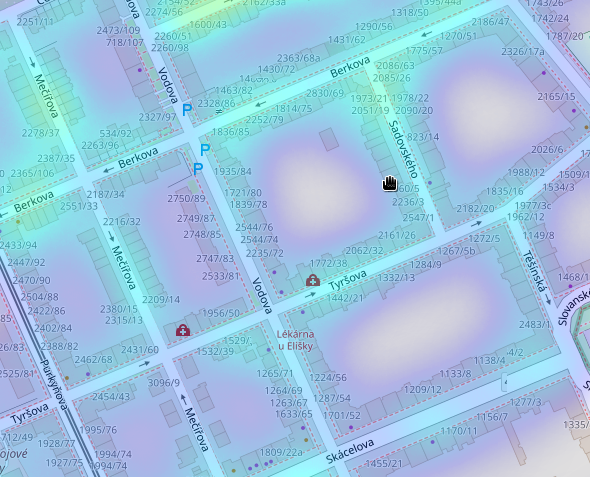
\includegraphics[width=0.6\linewidth]{obrazky-figures/brno-zastavana-oblast.png}
    \caption{Heat vrstva zastavanej časti Brna.}
    \label{fig:brno-zastavana-oblast}
\end{figure}

\textbf{Heat vrstva pre polygóny} by mala mať väčší rádius. Nestačí, keď sa pre polygón vytvorí vrstva iba vo~vnútornej časti budovy, vrstva by mala mať takú istú hodnotu aj~v~najbližšej oblasti budovy. Na obrázku~\ref{fig:nechov-bad-heatmap} je vidieť, že časť polygónov je bez vytvorenej heat vrstvy a~takisto aj~najbližšie okolie polygónov je bez tejto vrstvy.

\begin{figure}[ht]
    \centering
    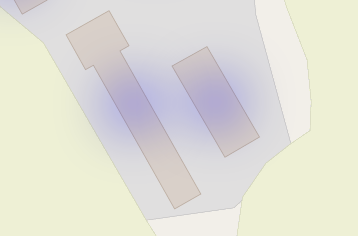
\includegraphics[width=0.3\linewidth]{obrazky-figures/nechov-zle-vykreslenie.png}
    \caption{Heat vrstva by sa mala vykresliť aj vo~vonkajšej časti polygónov.}
    \label{fig:nechov-bad-heatmap}
\end{figure}

\textbf{Cesta medzi dvoma významnými objektami} by mala mať vyššiu hodnotu pravdepodobnosti. Napríklad ak si predstavíme cestu medzi školou a~autobusovou stanicou (obidva objekty majú pravdepodobnosť 1.0), tak vieme, že na~takejto ceste by mala byť pre danú cestu vyššia pravdepodobnosť výskytu osôb. Možným riešením by bolo použiť pri vytváraní vrstvy kataster nehnuteľností alebo územný plán obce.

\textbf{Nepresnosti v~získaných mapových dátach} vytvára na~mape body heat vrstvy, ktoré by sa nemali s~vytvorenou vrstvou zobrazovať. Aj~keď väčšina mapových dát zo~stráky Geofabrik býva aktualizovaná  
každý deň, aj tak sa v~týchto mapových dátach vyskytujú chyby. Takéto potenciálne chyby by sa dali odstrániť pridaním možnosti užívateľovi upravovať vytvorenú heat vrstvu. Funkcionalita takejto vlastnosti by sa dala implementovať pomocou vytvárania heat vrstvy myšou alebo pridávaním a~odstraňovaním bodov heat vrstvy z~mapy pomocou vstupného formulára.



\chapter{Záver}
\label{chap:zaver}
Cieľom tejto bakalárskej práce bolo vytvoriť aplikáciu, ktorá na~základe získaných dát vytvorí heat mapu pravdepodobnosti výskytu osôb v~určitej oblasti. Aplikáciu sa podarilo úspešne vytvoriť s~miernymi nedostatkami.

Pred začatím implementácie bolo potrebné sa zoznámiť s~potrebnou teóriou. Obsahom teórie boli zdroje mapových dát a~spôsoby ich reprezentácie. Zistil som, že mapové dáta môžu byť reprezentované v~rastrovom formáte alebo vo~vektorovom formáte a~tieto formáty majú rôzne formáty súborov, ktorými môžu byť reprezentované. Pri implementácii boli použité mapové dáta vo~vektorovom formáte, pretože poskytujú informácie o~jednotlivých geografických objektoch na~mape. Potom bolo nutné naštudovať, aké sú možnosti dolovania dát z~volne dostupných zdrojov. Zistil som, že najjednoduchším spôsobom je získavanie dát zo~stránok projektu OpenStreetMap.

Pri implementácii boli zvolené vhodné technológie, ktoré vyšli z~návrhu aplikácie. Samotná aplikácia pozostáva z~primárnej funkcionality a~z~užívateľského rozhrania. Primárnu funkcionalitu zahŕňa získanie dát a~ich spracovanie pomocou knižnice GeoPandas do~dvojrozmernej dátovej štruktúry. Vytvorený dátový rámec obsahuje geografické objekty a~tie sa využívajú spoločne so~získanými pravdepodobnosťami na vytvorenie heat vrstvy na~mape pomocou knižnice Leaflet. Takáto vytvorená heat vrstva na~mape reprezentuje pravdepodobný odhad výskytu osôb v~určitej oblasti.

Vypracovaním tejto bakalárskej práce som spoznal, ako je možné získavať mapové dáta a ako sú reprezentované na~mape. Počas testovania aplikácie som narazil na~viacero problémov. Preto by som chcel v~práci pokračovať a~vylepšiť aplikáciu o~lepšie zobrazovanie heat vrstvy u~rôznych geografických objektoch. Určite by som chcel zlepšiť vytváranie heat vrstvy u~polygónov, aby zobrazená vrstva bola aj~v~okolí zobrazeného polygónu na~mape. Ďalším možným vylepšením by bolo pridanie viacerých parametrov, ktoré by mohol užívateľ zadať. Teda okrem hodnoty pravdepodobnosti pre danú značku by mohol zadať napríklad aj~veľkosť priemeru kruhu heat bodov pre daný geografický objekt.
